\documentclass[12pt, twoside]{article}
\usepackage{jmlda}
\usepackage{graphicx}
\newcommand{\hdir}{.}

% notations
% bold
\newcommand{\bz}{\mathbf{z}}
\newcommand{\bx}{\mathbf{x}}
\newcommand{\by}{\mathbf{y}}
\newcommand{\bw}{\mathbf{w}}
\newcommand{\bfx}{\mathbf{f}}
\newcommand{\bb}{\mathbf{b}}
\newcommand{\bu}{\mathbf{u}}
\newcommand{\bh}{\mathbf{h}}
\newcommand{\bX}{\mathbf{X}}
\newcommand{\bZ}{\mathbf{Z}}
\newcommand{\bA}{\mathbf{A}}
\newcommand{\bI}{\mathbf{I}}
\newcommand{\bJ}{\mathbf{J}}
\newcommand{\bV}{\mathbf{V}}
\newcommand{\bU}{\mathbf{U}}
\newcommand{\bG}{\mathbf{G}}
\newcommand{\btheta}{\boldsymbol{\theta}}
\newcommand{\bPsi}{\boldsymbol{\Psi}}
\newcommand{\bpsi}{\boldsymbol{\psi}}
\newcommand{\bxi}{\boldsymbol{\xi}}
\newcommand{\bchi}{\boldsymbol{\chi}}
\newcommand{\bzeta}{\boldsymbol{\zeta}}
\newcommand{\blambda}{\boldsymbol{\lambda}}
\newcommand{\beps}{\boldsymbol{\varepsilon}}
\newcommand{\bZeta}{\boldsymbol{Z}}
\newcommand{\bg}{\mathbf{g}}
\newcommand{\bff}{\mathbf{f}}
\newcommand{\bv}{\mathbf{v}}
% mathcal
\newcommand{\cX}{\mathcal{X}}
\newcommand{\cY}{\mathcal{Y}}
\newcommand{\cW}{\mathcal{W}}
\newcommand{\cL}{\mathcal{L}}
% transpose
%\newcommand{\T}{^{\mathsf{T}}}
%other
\newcommand{\fD}{\mathfrak{D}}
\newcommand{\fG}{\mathfrak{G}}
\newcommand{\fF}{\mathfrak{F}}
\newcommand{\bbR}{\mathbb{R}}
\newcommand{\bbY}{\mathbb{Y}}

\begin{document}

\title
    [Оптимизация параметров модели на основе дистилляции знаний] % краткое название; не нужно, если полное название влезает в~колонтитул
    {Регуляризация траектории параметров модели глубокого обучения на основе дистилляции знаний}
\author
    [М.~Горпинич] % список авторов (не более трех) для колонтитула; не нужен, если основной список влезает в колонтитул
    {М.~Горпинич, О.\,Ю.~Бахтеев, В.\,В.~Стрижов} % основной список авторов, выводимый в оглавление
    [М.~Горпинич, О.\,Ю.~Бахтеев, В.\,В.~Стрижов] % список авторов, выводимый в заголовок; не нужен, если он не отличается от основного
\email
    {gorpinich4@gmail.com; bakhteev@phystech.edu;  strijov@ccas.ru}
%\thanks
%    {Работа выполнена при
%     частичной
%     финансовой поддержке РФФИ, проекты \No\ \No 00-00-00000 и 00-00-00001.}
%\organization
%    {$^1$Организация, адрес; $^2$Организация, адрес}
\abstract
    {Исследуется задача оптимизации параметров модели глубокого обучения. Во время оптимизации также учитывается информация, содержащаяся в модели с более сложной структурой, то есть применяется дистилляция. Предлагается обобщение методов дистилляции, заключающееся в градиентной оптимизации метапараметров. Под метапараметрами модели понимаются параметры оптимизационной задачи дистилляции, а именно, коэффициенты перед слагаемыми в функции ошибки и температура. Функция ошибки состоит из двух слагаемых: правдоподобия исходной выборки и правдоподобия выборки дистилляции. Температурой является коэффициент, на который домножаются логиты моделей при применении функции softmax. Исследуются свойства оптимизационной задачи и методы предсказания траектории оптимизации метапараметров модели. Данное обобщение дистиллирует модель с лучшими эксплуатационными характеристиками и за меньшее число итераций оптимизации. Проиллюстрирован данный подход с помощью вычислительного эксперимента на выборке CIFAR-10 и на синтетической выборке.
	
\bigskip
\noindent
\textbf{Ключевые слова}: \emph {машинное обучение; дистилляция знаний; оптимизация метапараметров}
}

\titleEng
	[Model parameter optimization with knowledge distillation] % краткое название; не нужно, если полное название влезает в~колонтитул
    {Regularizing optimization trajectory of deep learning model parameters with knowledge distillation}
\authorEng
	[M.~Gorpinich] % список авторов (не более трех) для колонтитула; не нужен, если основной список влезает в колонтитул
    {M.~Gorpinich, O.\,Yu.~Bakhteev, V.\,V.~Strijov} % основной список авторов, выводимый в оглавление
    [M.~Gorpinich, O.\,Yu.~Bakhteev, V.\,V.~Strijov] % список авторов, выводимый в заголовок; не нужен, если он не отличается от основного

\abstractEng
{The paper investigates parameter optimization problem for deep learning neural networks. The knowledge of a cumbersome model is considered during optimization, i.e. the knowledge distillation is used. The paper proposes generalization of knowledge distillation method to optimize meta-parameters by gradient descent. Meta-parameters are the parameters of knowledge distillation optimization problem, namely, the coefficients before terms in error function and the temperature factor. The error function is a sum of likelihood of the initial dataset and the one of distillation dataset. Temperature is a factor of logits of models in softmax function. The authors investigate the properties of optimization problem and methods to predict the optimization path of meta-parameters. Generalized method produces models with higher performance and uses less number of iterations. The algorithm is evaluated on CIFAR-10 dataset and synthetic data.


\noindent
\textbf{Keywords}: \emph{machine learning; knowledge distillation; metaparameter optimization}}

%данные поля заполняются редакцией журнала
\doi{}
\receivedRus{}
\receivedEng{}

\maketitle
\linenumbers

\section{Введение}
В работе исследуется проблема оптимизации моделей глубоких нейросетей. Данная оптимизация требует значительных вычислительных мощностей и является затратной по времени. В данной работе предлагается метод оптимизации, позволяющий улучшить точность предсказаний модели, а также ускорить сходимость траектории оптимизации параметров к точке оптимума.

Предлагается обобщение метода оптимизации на основе дистилляции знаний. Назовем \textit{дистилляцией знаний} задачу оптимизации параметров модели прогнозирования, при которой учитывается не только информация, содержащаяся в выборке, но также и информация, содержащаяся в сторонней модели (модели-учителе). Рассматривается \textit{модель-учитель} более сложной структуры, которая была обучена на выборке. Модель более простой структуры предлагается оптимизировать путем переноса знаний модели учителя на более простую модель, называемую \textit{моделью-учеником}. При этом ее качество будет выше по сравнению с качеством, полученным после оптимизации на той же выборке. Данный подход описан в~\cite{journals/corr/HintonVD15}. В~\cite{conf/cvpr/PassalisTT20} предложен подход к дистилляции знаний, переносящий знания на модель с архитектурой, значительно отличающейся от архитектуры модели-учителя.

Предлагается формулировка задачи в виде двухуровневой оптимизации. На первом уровне оптимизируются параметры модели, на втором уровне --- ее метапараметры. Данный подход описан в~\cite{journals/corr/LuketinaBR15, journals/anor/BakhteevS20, journals/corr/MaclaurinDA15}. В~\cite{journals/corr/LuketinaBR15} рассматривается жадный градиентный метод оптимизации метапараметров. В~\cite{journals/anor/BakhteevS20} сравниваются различные градиентные методы оптимизации метапараметров, а также метод случайного поиска.

В работе рассматривается подход к прогнозированию значений метапараметров, полученных методом градиентной оптимизации. Под метапараметрами понимаются параметры задачи оптимизации. Сложность градиентной оптимизации для метапараметров является квадратичной по числу параметров, и потому вычислительно затратна. Предлагается аппроксимация траектории оптимизации метапараметров на основе приближения траектории линейной моделью. Вычислительный эксперимент проводится на выборке изображений CIFAR-10~\cite{krizhevsky2009learning}, а также синтетической выборке.

\section{Постановка задачи}
Решается задача классификации вида:

\begin{equation} \label{eq:data}
    \fD = \{(\bx_i, y_i)\}_{i=1}^{m},\; \bx_i \in \bbR^n,\; y_i \in \bbY = \{1, \dots, K\},
\end{equation}

\noindent
где~$y_i$ — это класс объекта, также будем обозначать~$\by_i$ вектором вероятности для
класса~$y_i$.

Разобьем выборку следующим образом:

\begin{equation} \label{eq:split}
    \fD = \fD_\text{train} \sqcup \fD_\text{val}.
\end{equation}

Подвыборку~$\fD_\text{train}$ будем использовать для оптимизации параметров модели, а подвыборку~$\fD_\text{val}$ --- для оптимизации метапараметров.

Внешним критерием качества назначена доля правильных ответов:

\begin{equation} \label{eq:accuracy}
    \text{accuracy} = \frac{1}{m}\sum\limits_{i=1}^m [\bg(\bx_i, \bw) = y_i],
\end{equation}

\noindent
где~$\bg$ --- параметрическая модель классификации с параметрами~$\bw$.

\textbf{Определение 1.}
Назовем \textit{дистилляцией знаний} задачу оптимизации параметров модели прогнозирования, при которой учитывается не только информация, содержащаяся в выборке, но также и информация, содержащаяся в сторонней модели (модели-учителе).

Зафиксирована модель учителя~$\bff$. Функция потерь~$\cL_\text{train}$, в которой учитывается перенос информации от модели учителя~$\bff$ к модели ученика~$\bg$, имеет вид:

\begin{equation} \label{eq:l_train}
    \cL_\text{train}(\bw, \boldsymbol{\lambda}) = -\lambda_1\sum\limits_{(\bx, y) \in \fD_\text{train}}\underbrace{\sum\limits_{k=1}^{K}y^k\log \bg(\bx, \bw)|_{T=1}}_{\text{исходная функция потерь}} - \lambda_2\sum\limits_{(\bx, y) \in \fD_\text{train}}\underbrace{\sum\limits_{k=1}^{K}\bff(\bx)|_{T=T_0}\log \bg(\bx, \bw)|_{T=T_0}}_{\text{слагаемое дистилляции}},
\end{equation}

\noindent
где~$T$ --- параметр температуры. Параметр температуры~$T$ имеет следующие свойства:

\begin{itemize}
    \item[1)] при~$T \rightarrow 0$ получаем вектор, в котором один из классов имеет единичную вероятность;
    \item[2)] при~$T \rightarrow \infty$ получаем равновероятные классы.
\end{itemize}

\noindent
Выражение~$\cdot |_{T=t}$ обозначает, что параметр температуры~$T$ в предыдущей функции равняется~$t$.

Зададим множество метапараметров~$\boldsymbol{\lambda}$ как вектор, состоящий из температуры и коэффициента перед слагаемым дистилляции:

\[\boldsymbol{\lambda} = [\lambda_1, \lambda_2, T].\]

Итоговая оптимизационная задача:

\begin{equation} \label{eq:opt_hyp}
    \hat{\boldsymbol{\lambda}} = \argmax\limits_{\boldsymbol{\lambda} \in \bbR^3} \cL_\text{val}(\hat{\bw}, \boldsymbol{\lambda}),
\end{equation}

\begin{equation} \label{eq:opt_param}
    \hat{\bw} = \argmin\limits_{\bw \in \bbR^s} \cL_\text{train}(\bw, \boldsymbol{\lambda}),
\end{equation}

\noindent
где функция~$\cL_\text{val}$ определяется как: 
 \begin{equation} \label{eq:l_val}
     \cL_\text{val}(\bw, \boldsymbol{\lambda}) = \sum\limits_{(\bx, y) \in \fD_\text{val}}\sum\limits_{k=1}^{K}y^k\log \bg(\bx, \bw)|_{T=1}.
 \end{equation}

\textbf{Определение 2.} Назовем \emph{оператором оптимизации} алгоритм~$U$ выбора вектора параметров~$\bw^\prime$ по параметрам предыдущего шага~$\bw$:

\begin{equation*}
    \bw^\prime = U(\bw).
\end{equation*}

Оптимизируем параметры~$\bw$ при помощи~$\eta$ шагов оптимизации:

\begin{equation} \label{eq:oper_superp}
    \hat{\bw} = U \circ U \circ \dots \circ U(\bw_0, \boldsymbol{\lambda}) = U^\eta(\bw_0, \boldsymbol{\lambda}),
\end{equation}

\noindent
где~$\bw_0$ --- начальное значение вектора параметров~$\bw$,~$\boldsymbol{\lambda}$ --- совокупность метапараметров модели.

Переопределим задачу минимизации согласно определению оператора~$U$:

\begin{equation} \label{eq:hyp_oper}
    \hat{\boldsymbol{\lambda}} = \argmax\limits_{\boldsymbol{\lambda} \in \bbR^3} \cL_\text{val}\bigl(U^\eta(\bw_0, \boldsymbol{\lambda})\bigr).
\end{equation}

Схема оптимизации метапараметров:

\begin{enumerate}
    \item Для каждого~$i = \overline{0, l}$, где~$l$ --- число итераций, используемых для оптимизации метапараметров.
    \item Решим задачу \eqref{eq:hyp_oper} и получим новое значение метапараметров~$\boldsymbol{\lambda}^\prime$.
    \item Положим~$\boldsymbol{\lambda} = \boldsymbol{\lambda}^\prime$.
\end{enumerate}

\section{Градиентные методы оптимизации}

Оптимизационную задачу \eqref{eq:opt_hyp} и \eqref{eq:opt_param} решает оператор градиентного спуска:

\begin{equation} \label{eq:operator}
    U(\bw, \boldsymbol{\lambda}) = \bw - \gamma\nabla\cL_\text{train}(\bw, \boldsymbol{\lambda}),
\end{equation}

\noindent
где~$\gamma$ — длина шага градиентного спуска.

\noindent
Используем метод градиентного спуска, который зависит только от значений параметров~$\bw$ на предыдущем шаге. На каждой итерации получим следующее значение метапараметров:

\begin{equation} \label{eq:hyp_alg}
    \boldsymbol{\lambda}^\prime = \boldsymbol{\lambda} - \gamma_{\boldsymbol{\lambda}}\nabla_{\boldsymbol{\lambda}}\cL_\text{val}(U(\bw, \boldsymbol{\lambda}), \boldsymbol{\lambda}) = \boldsymbol{\lambda} - \gamma_{\boldsymbol{\lambda}}\nabla_{\boldsymbol{\lambda}}\cL_\text{val}(\bw - \gamma\nabla\cL_\text{train}(\bw, \boldsymbol{\lambda}), \boldsymbol{\lambda}).
\end{equation}

Градиентная оптимизация является вычислительно затратной, поэтому предлагается аппроксимировать траекторию оптимизации модели. 

\noindent
Предлагается предсказывать траекторию изменения метапараметров модели (а конкретно, их градиенты) с помощью линейных сплайнов через определенное число итераций, а в остальное время использовать градиентные методы.

\section{Вычислительный эксперимент}

Целью эксперимента является проверка работоспособности предложенного метода дистилляции моделей, а также анализ полученных моделей и их метапараметров. Эксперимент проводится на двух выборках: синтетической модели и выборке CIFAR-10. Результаты данной работы и исходный код эксперимента опубликованы в~\cite{distknow} и могут быть проверены или использованы в дальнейшей работе.

\subsection{Эксперимент на синтетической выборке}
В эксперименте используется синтетическая выборка:

$$\fD = \{(\bx_i, y_i)\}_{i=1}^{m},\; x_{ij} \in \cN(0, 1),\; j=1, 2, x_{i3} = [\text{sign}(x_{i1})+\text{sign}(x_{i2})>0]$$
$$y_i = \text{sign}(x_{i1}*x_{i2}+\delta) \in \bbY,$$

\noindent
где~$\delta$ --- это шум. При этом размер выборки модели-ученика намного меньше размера выборки модели-учителя.

% \begin{figure}[!ht]
%     \centering
%     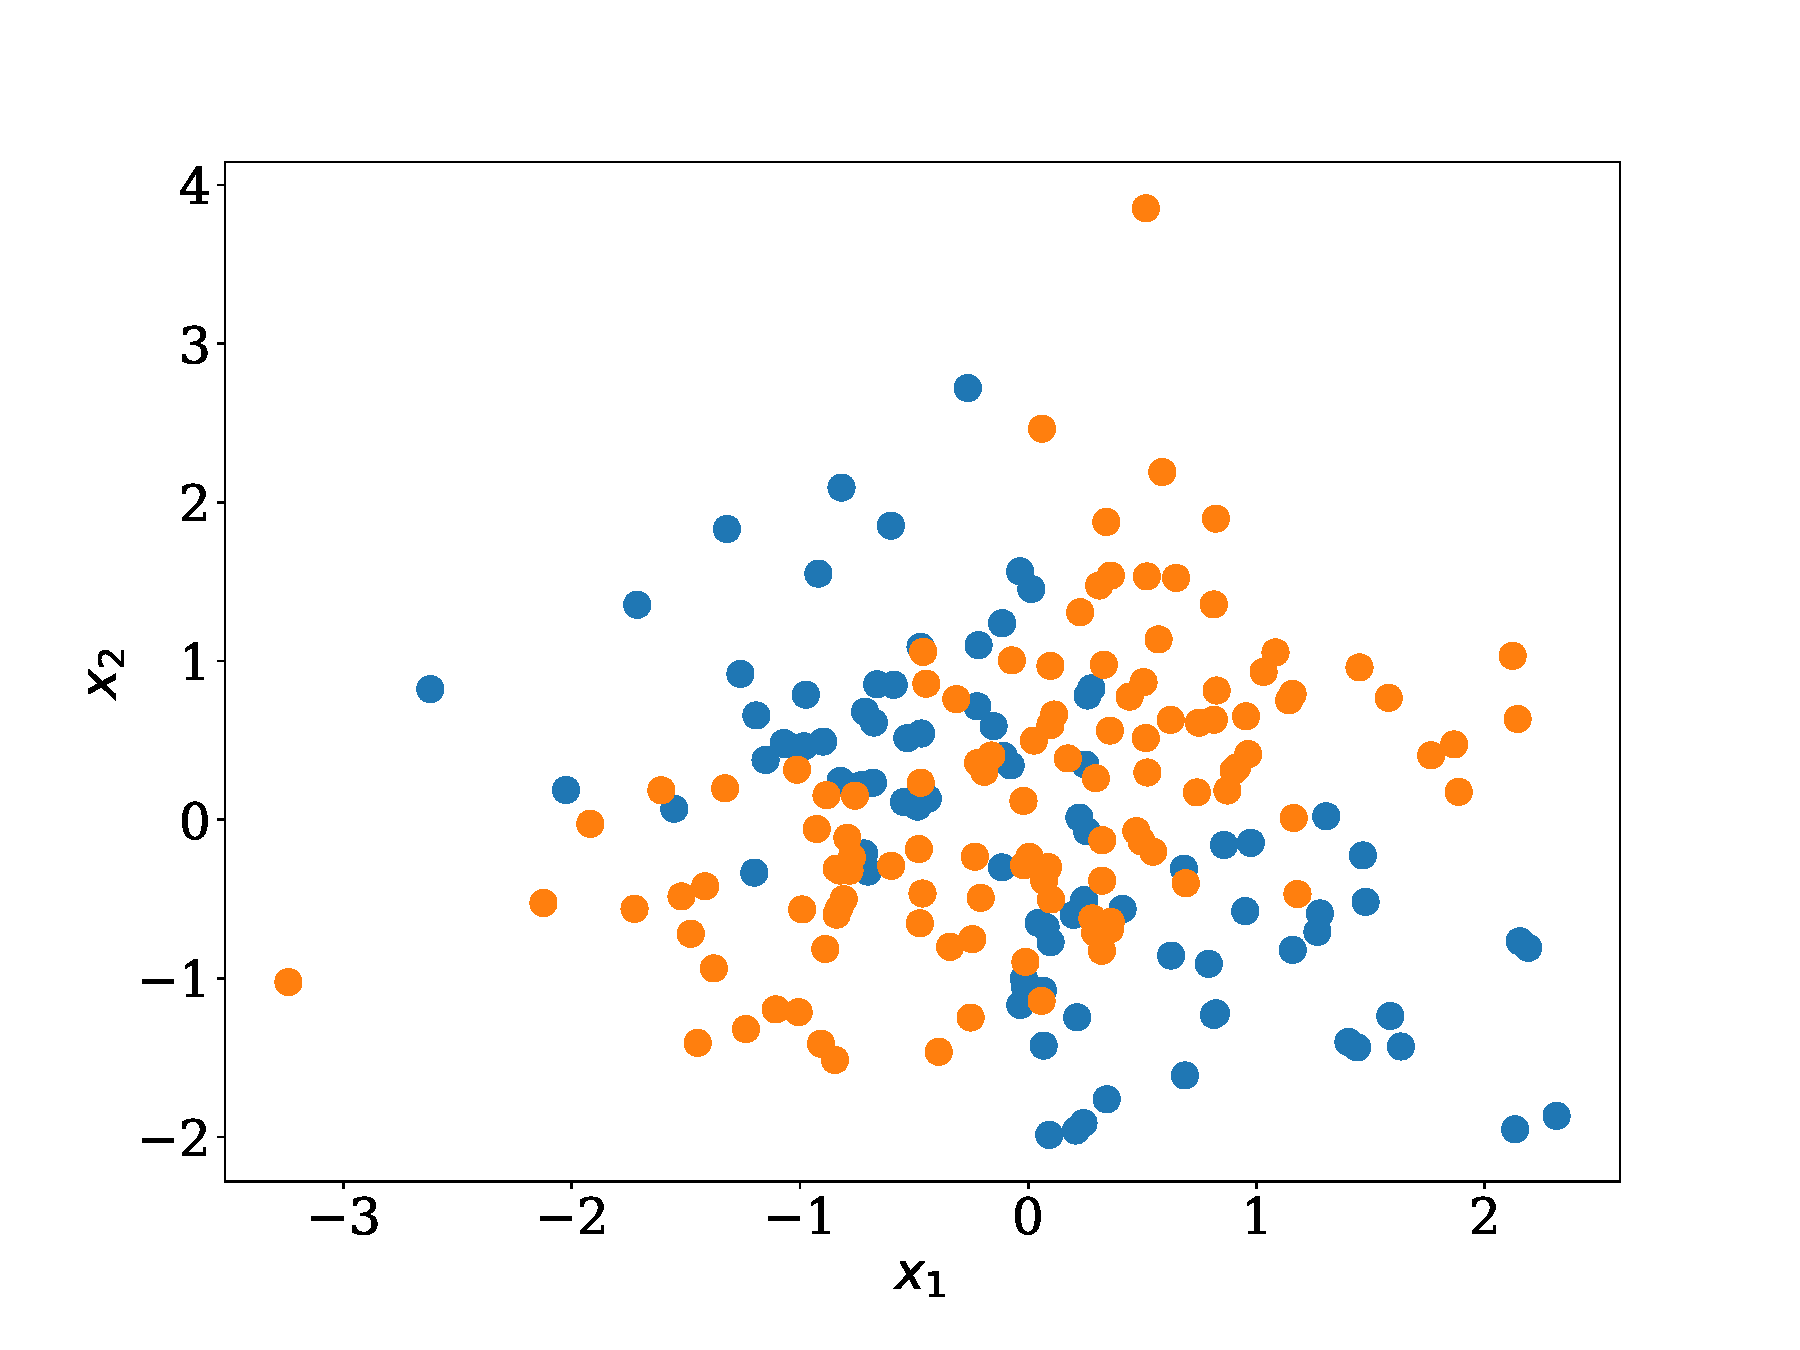
\includegraphics[width=0.6\textwidth]{ttrain.pdf}
%     \caption{Выборка для обучения учителя}
%     \label{fig:ttrain}
% \end{figure}

\begin{figure}[!ht]
% \center{
\begin{minipage}[h]{0.5\linewidth}
\center{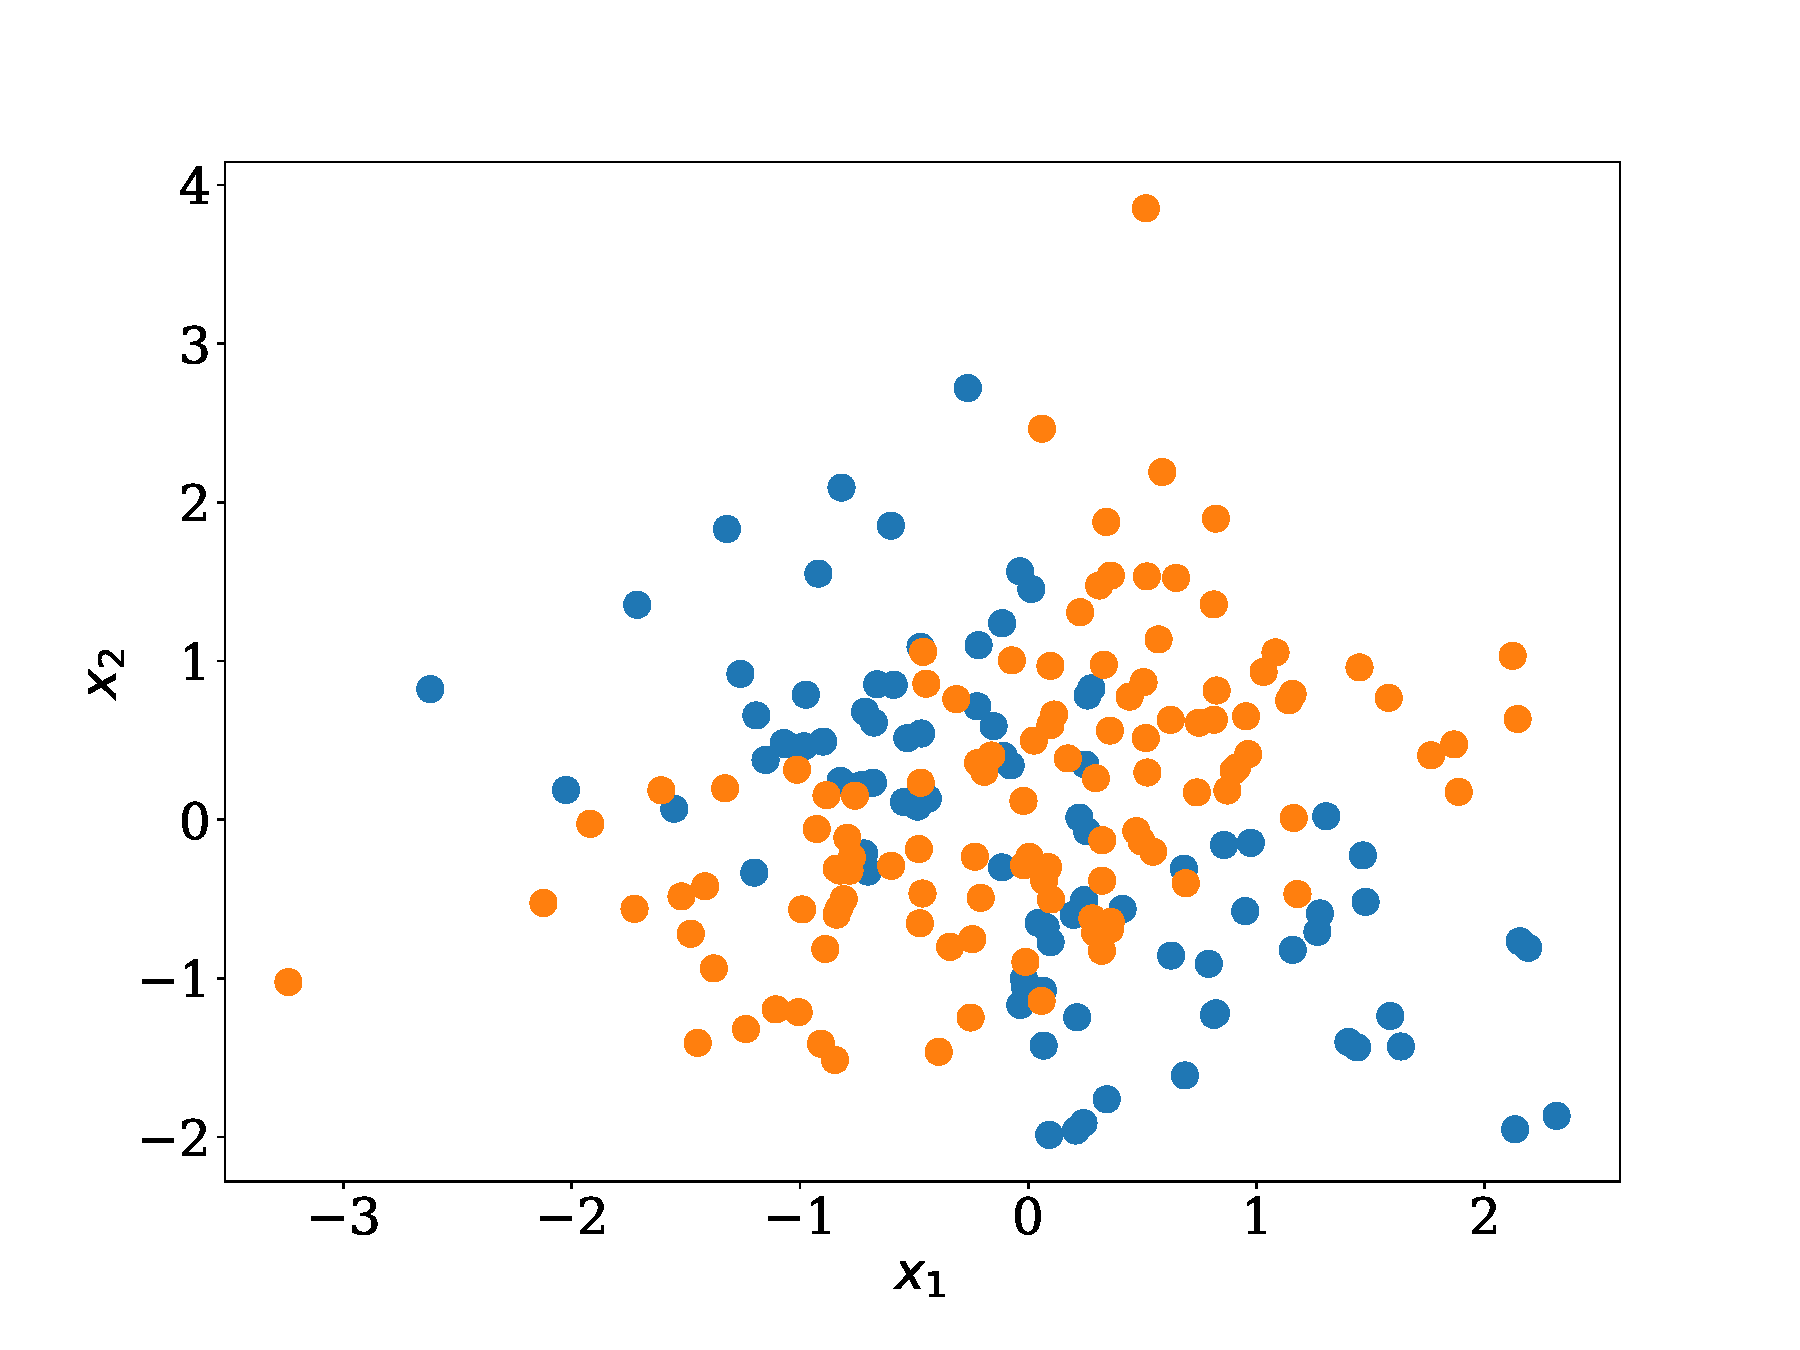
\includegraphics[width=\linewidth]{ttrain.pdf}\\а)}
\end{minipage}
\begin{minipage}[h]{0.5\linewidth}
\center{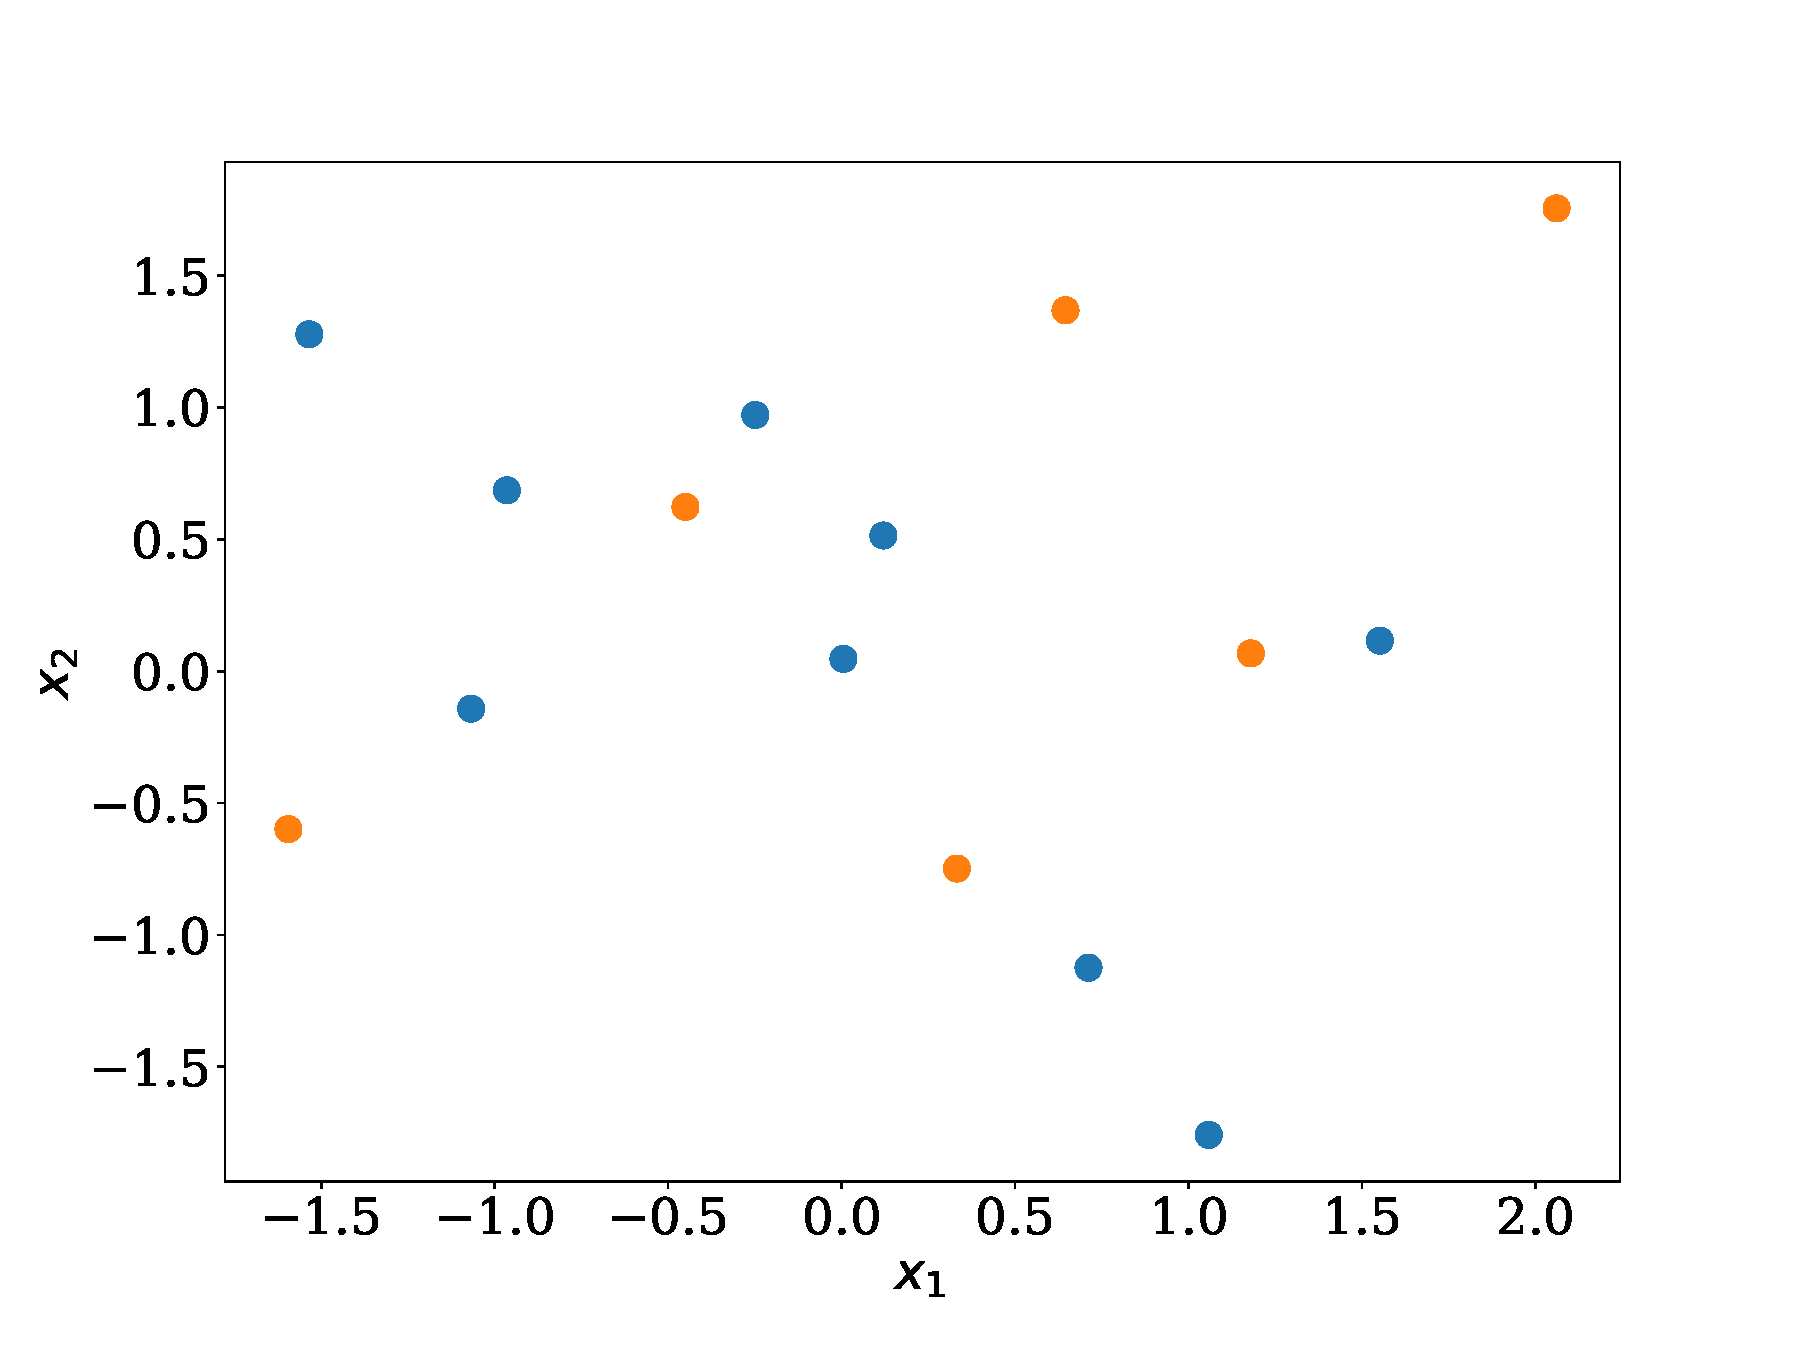
\includegraphics[width=\linewidth]{train.pdf}\\б)}
\end{minipage}
\center{
\begin{minipage}[h]{0.5\linewidth}
\center{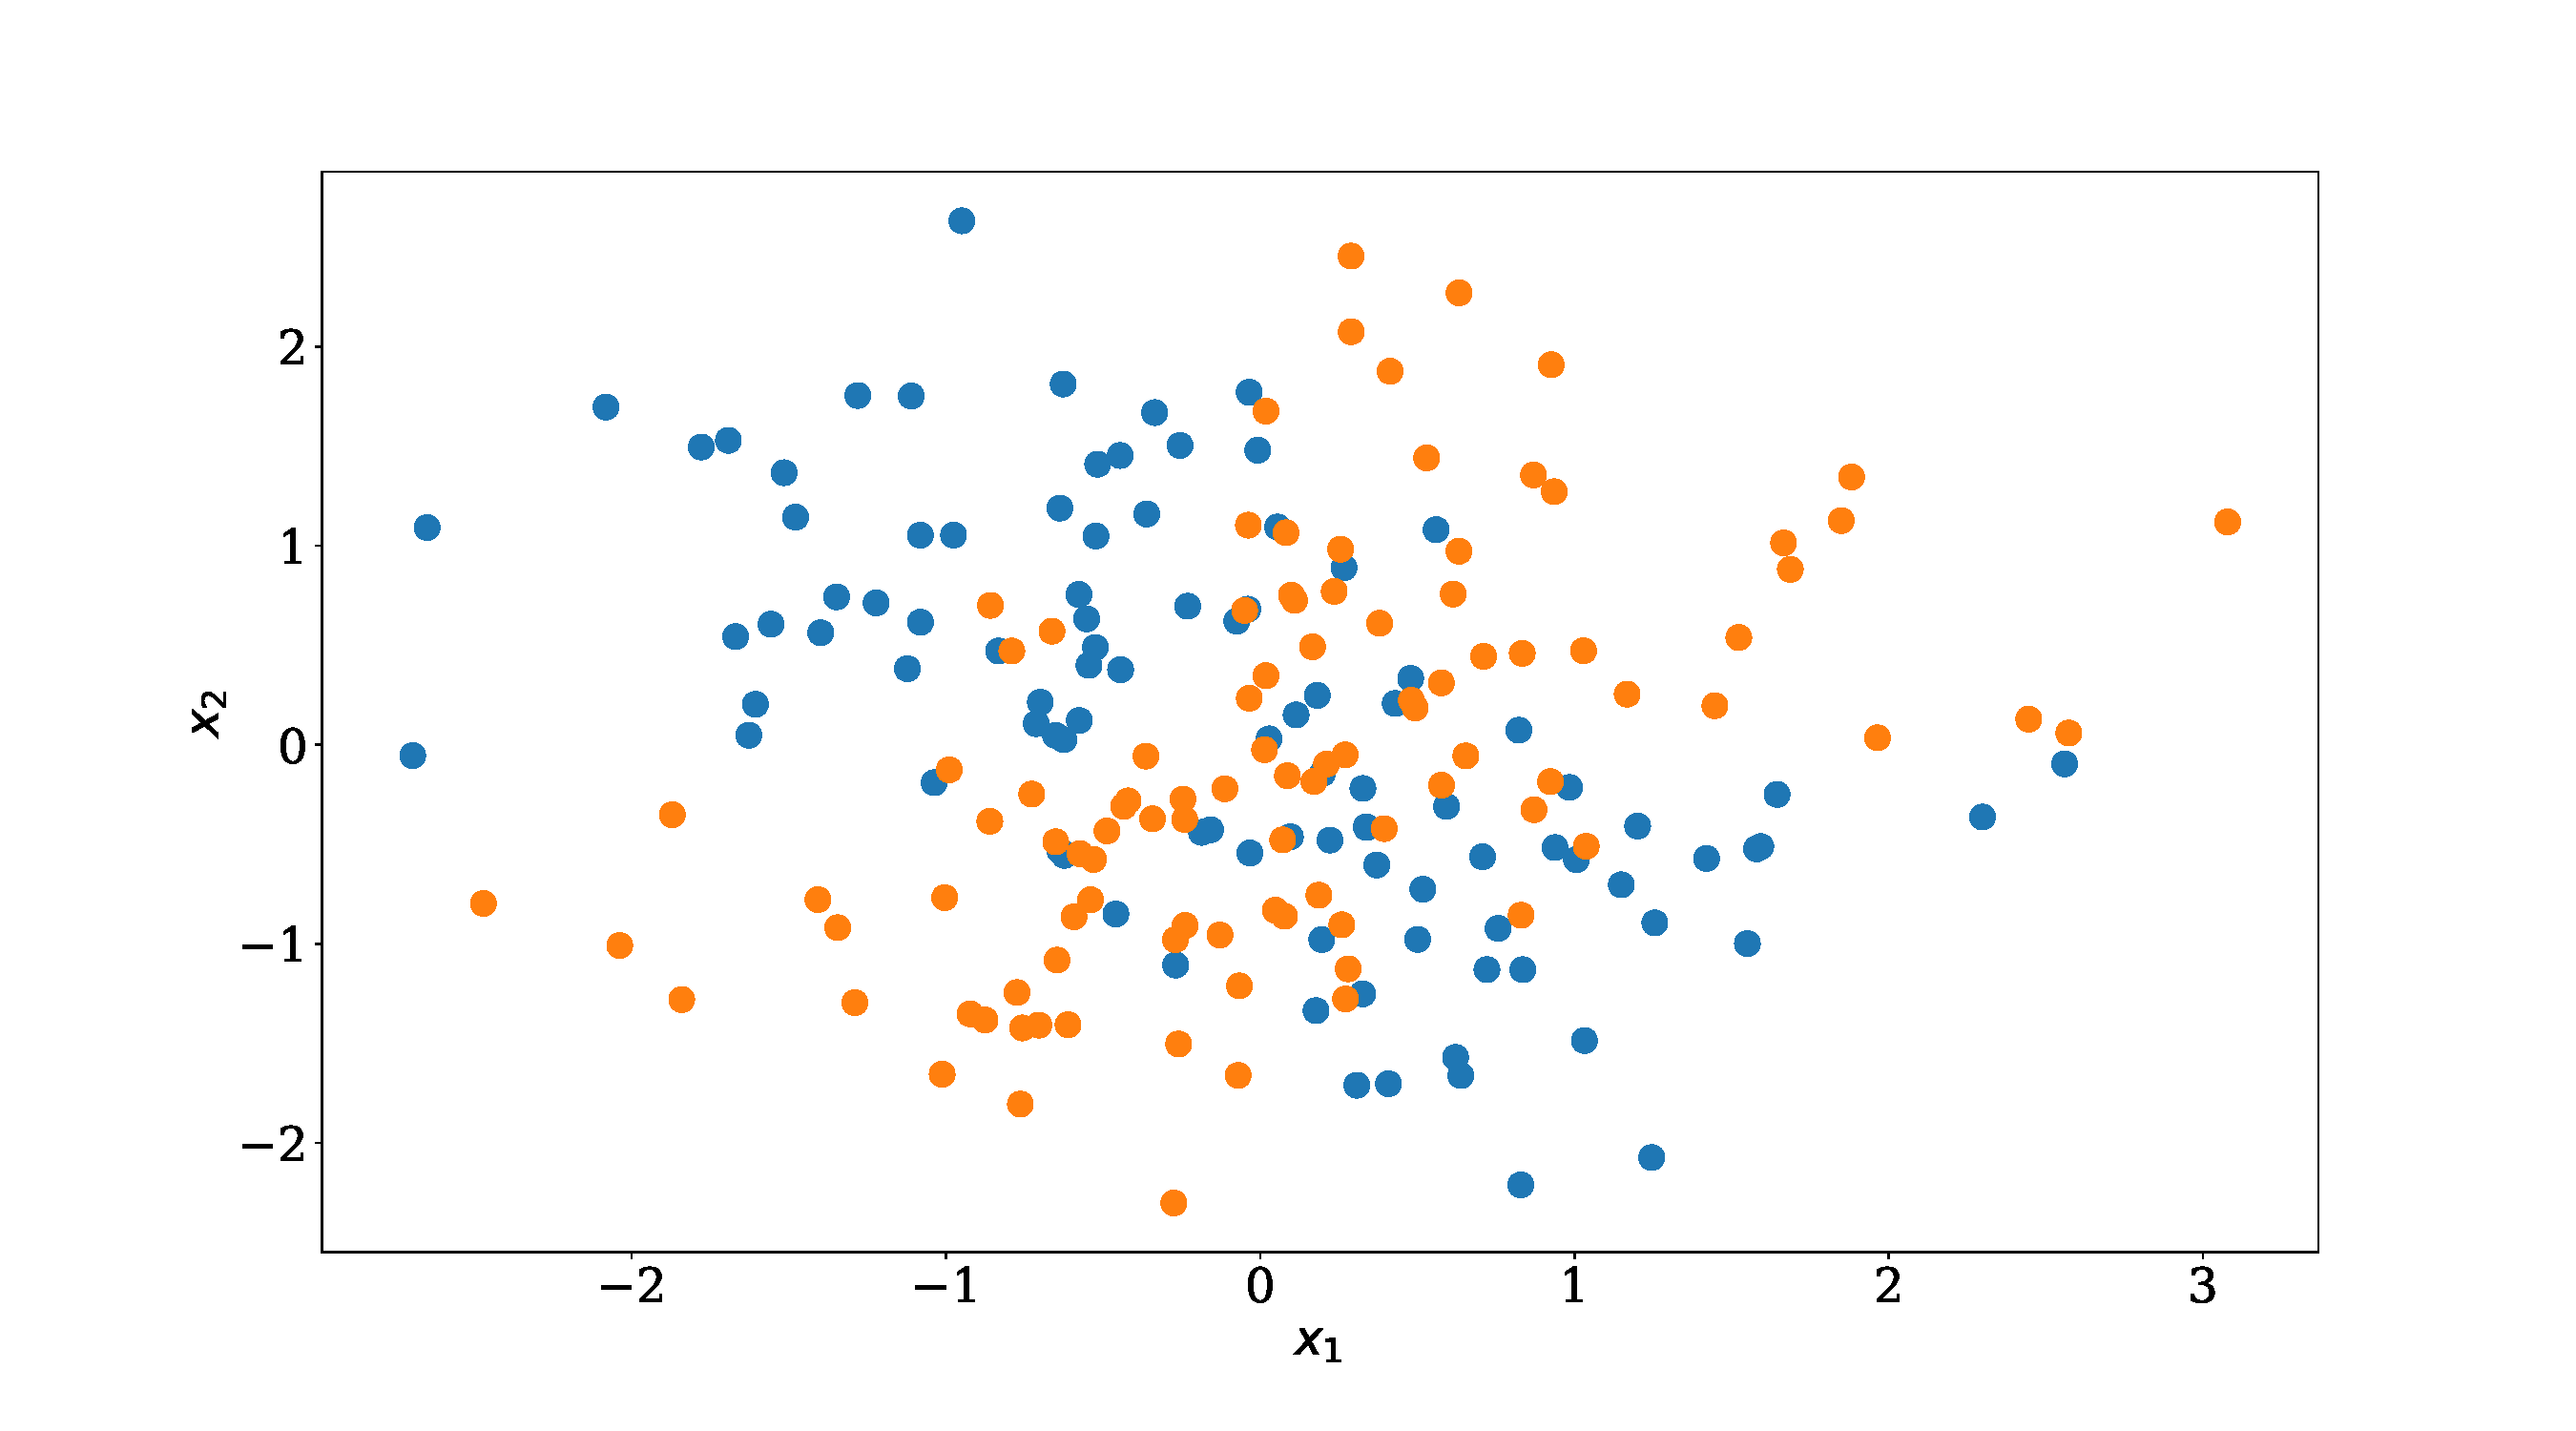
\includegraphics[width=\linewidth]{test.pdf}\\в)}
\end{minipage}}
\caption{Визуализация выборки а) для обучения учителя; б) для обучения ученика; в) тестовой выборки}
\label{fig:synt_data}
\end{figure}

% \begin{figure}[!ht]
%    \centering
%    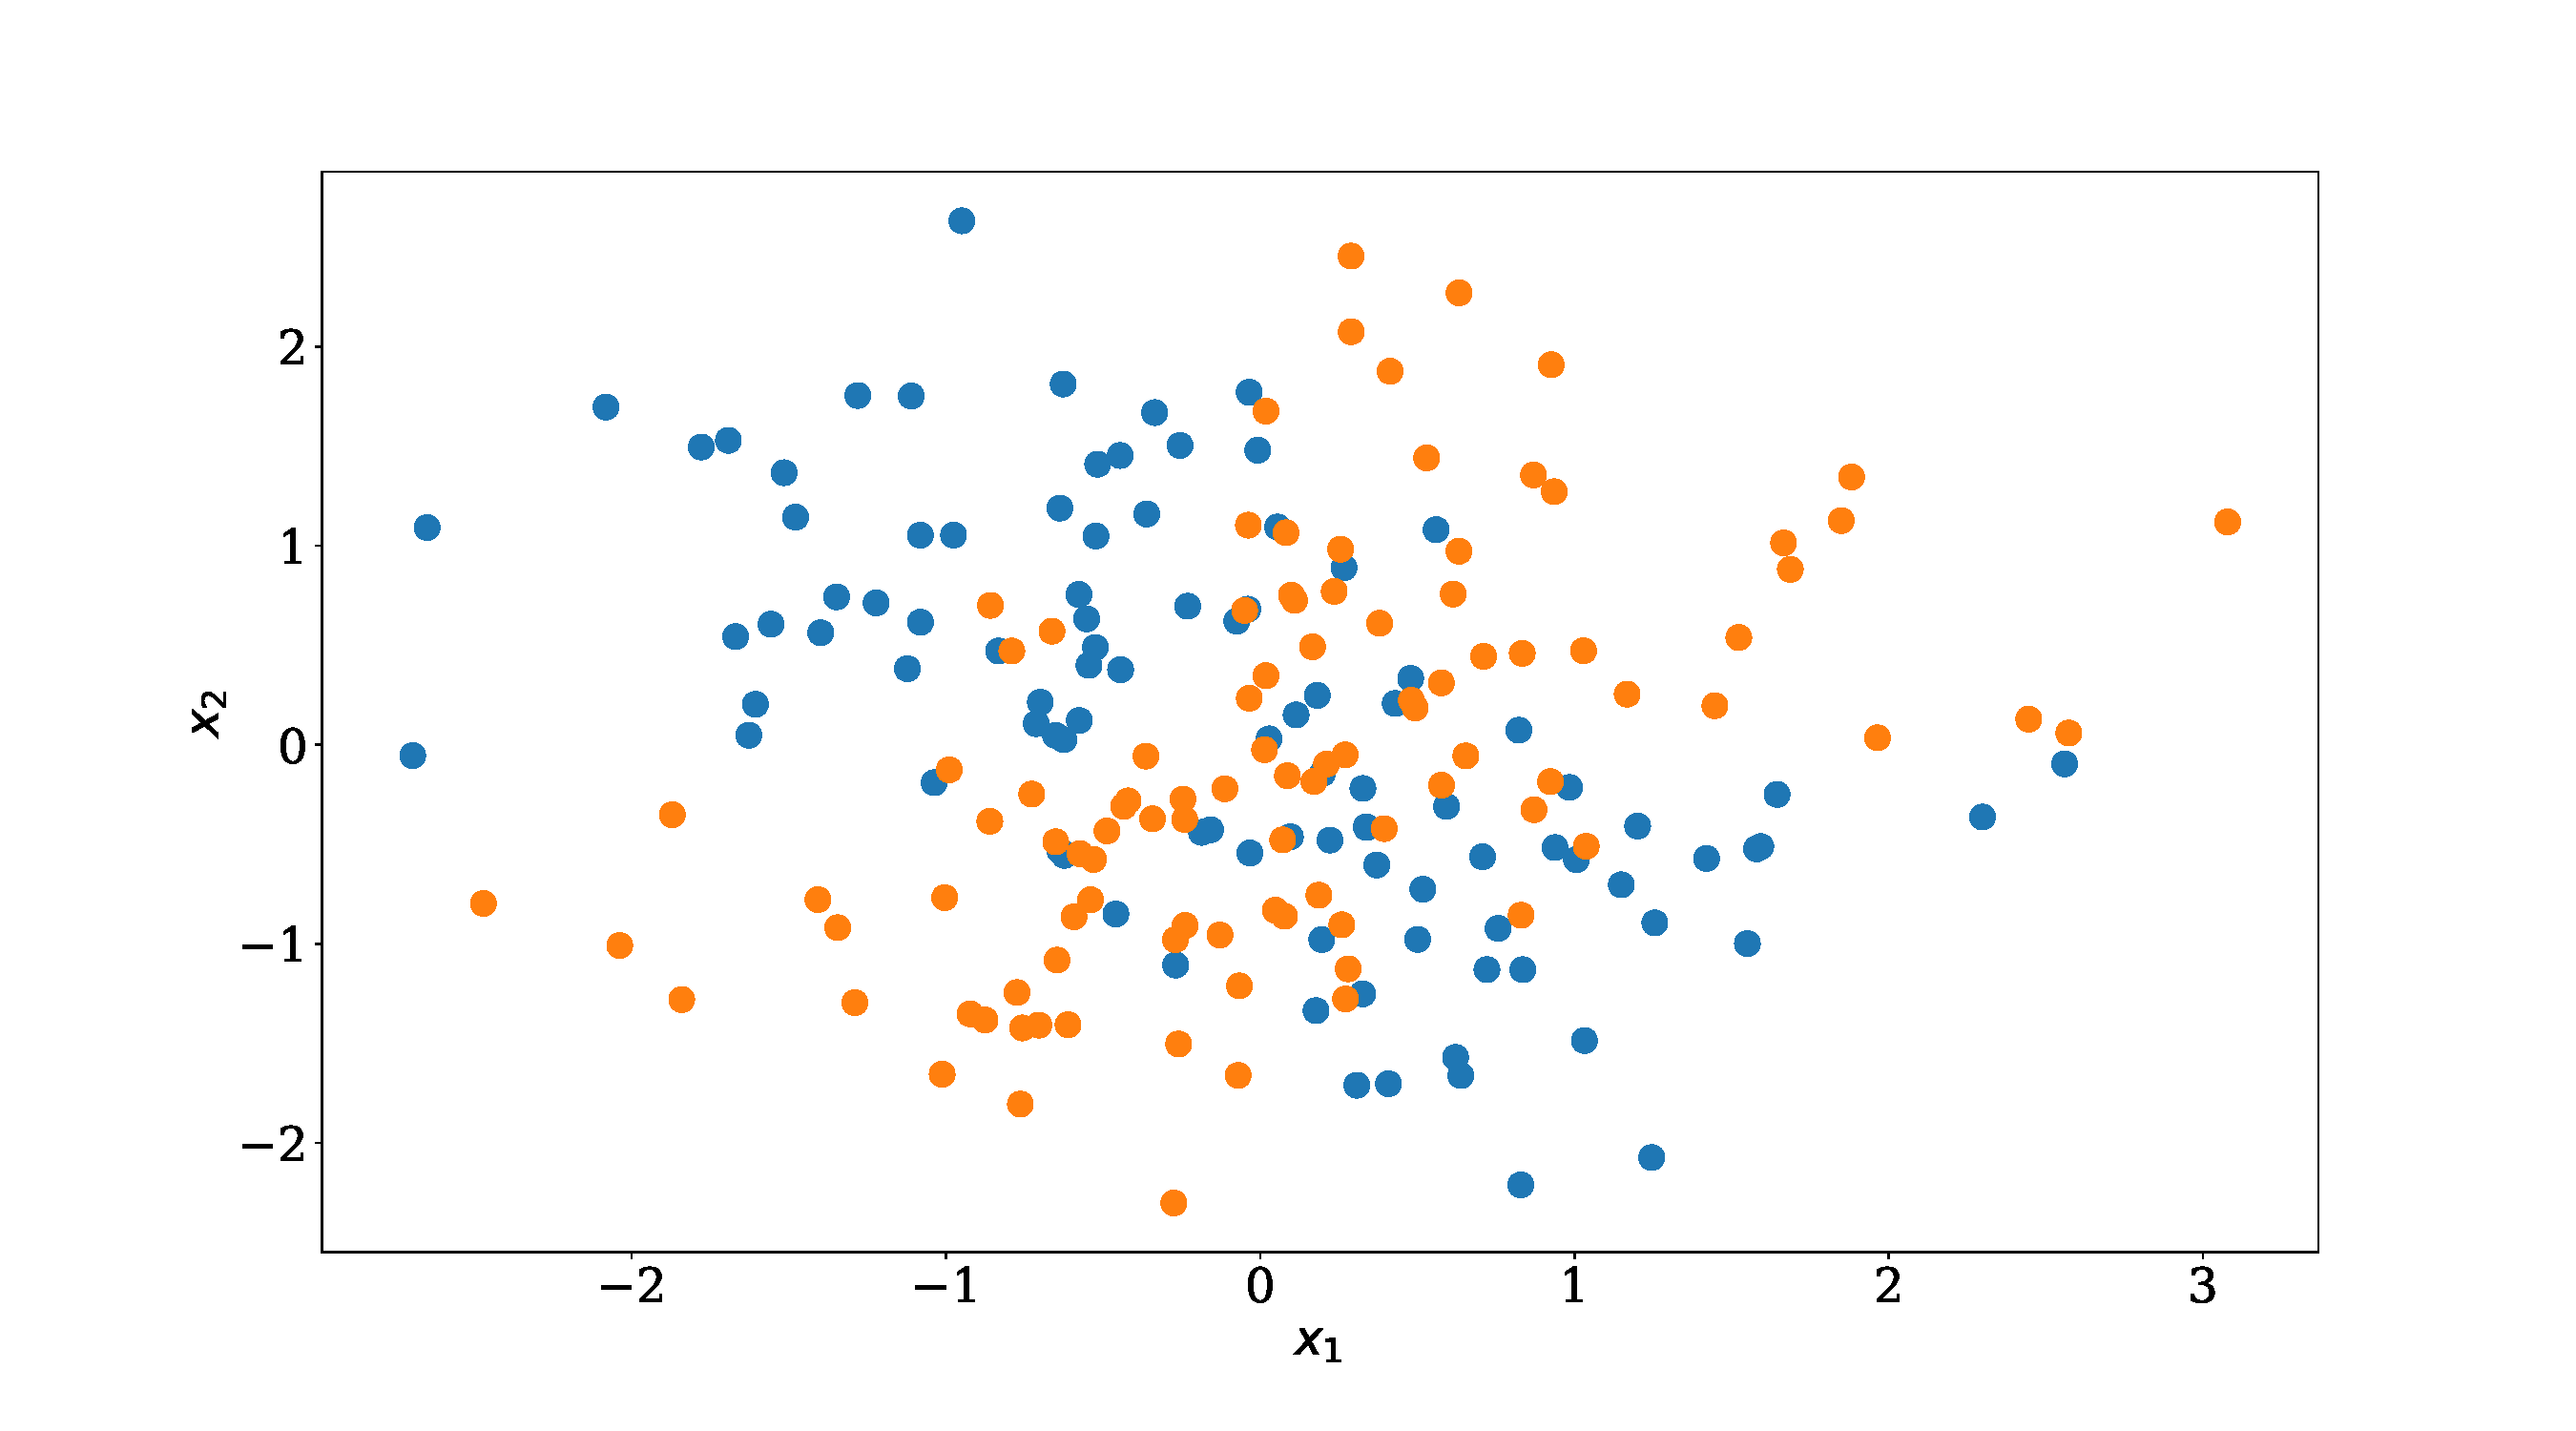
\includegraphics[width=0.6\textwidth]{test.pdf}
%    \caption{Тестовая выборка}
%    \label{fig:test}
% \end{figure}

Обучение модели-ученика проводилось несколькими методами: с использованием дистилляции и оптимизации метапараметров градиентными методами, дистилляции с предсказанием траектории оптимизации модели, дистилляции со случайными метапараметрами. При этом для обучения модели с использованием сплайнов дополнительно проводились серии экспериментов для определения наилучшего размера эпохи и наилучшего числа эпох между предсказаниями траектории с помощью сплайнов.

\begin{figure}[!ht]
\centering
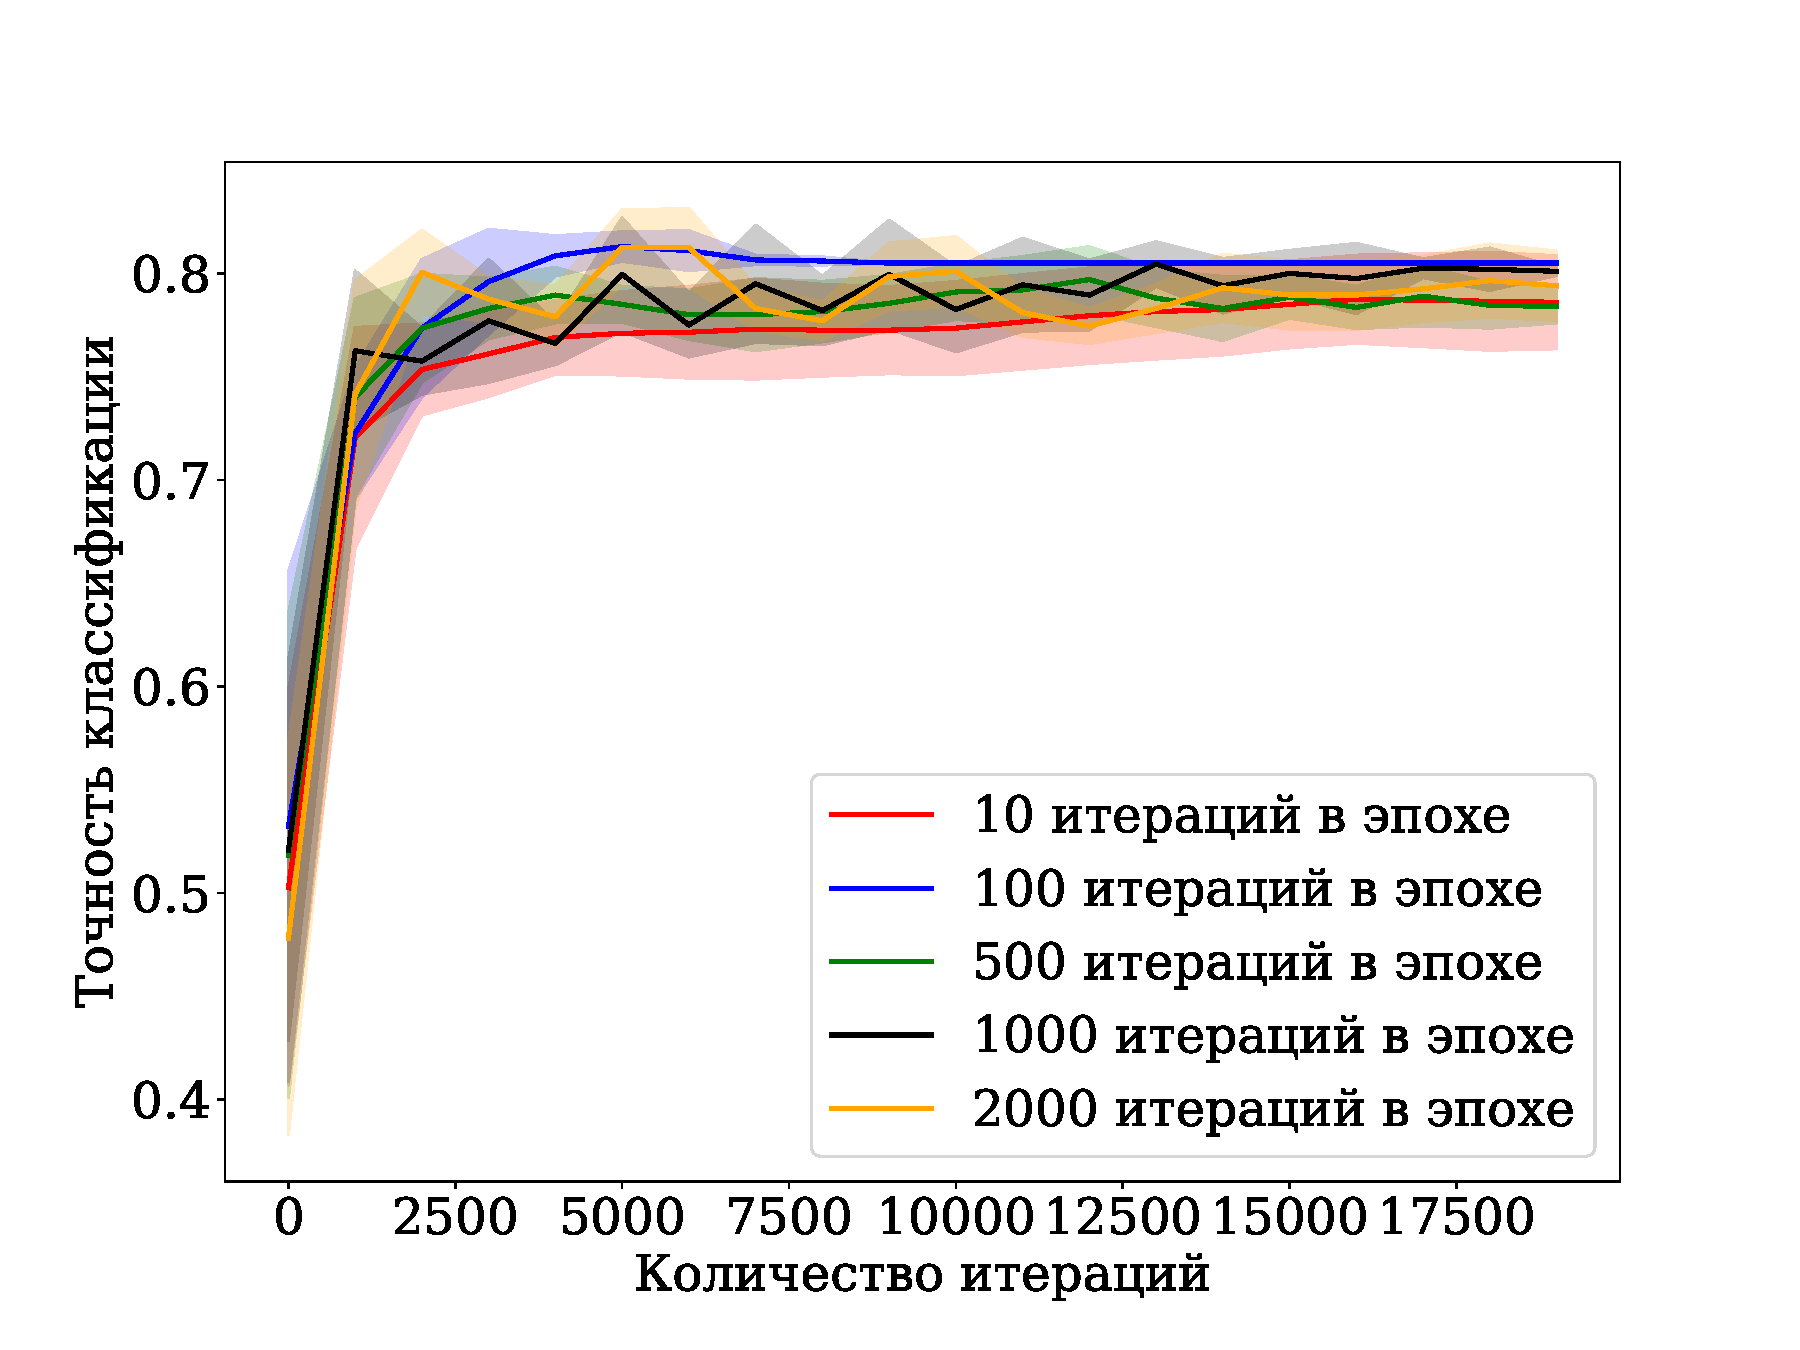
\includegraphics[width=0.6\textwidth]{linear_epoch_size.pdf}
\caption{График зависимости точности классификации от номера итерации при различных значениях размера эпохи}
\label{fig:epoch_size}
\end{figure}

На рис. \ref{fig:epoch_size} показан график зависимости точности от номера итерации при различных размерах эпохи. Согласно данному графику размер эпохи был выбран равным 100.

\begin{figure}[!ht]
\centering
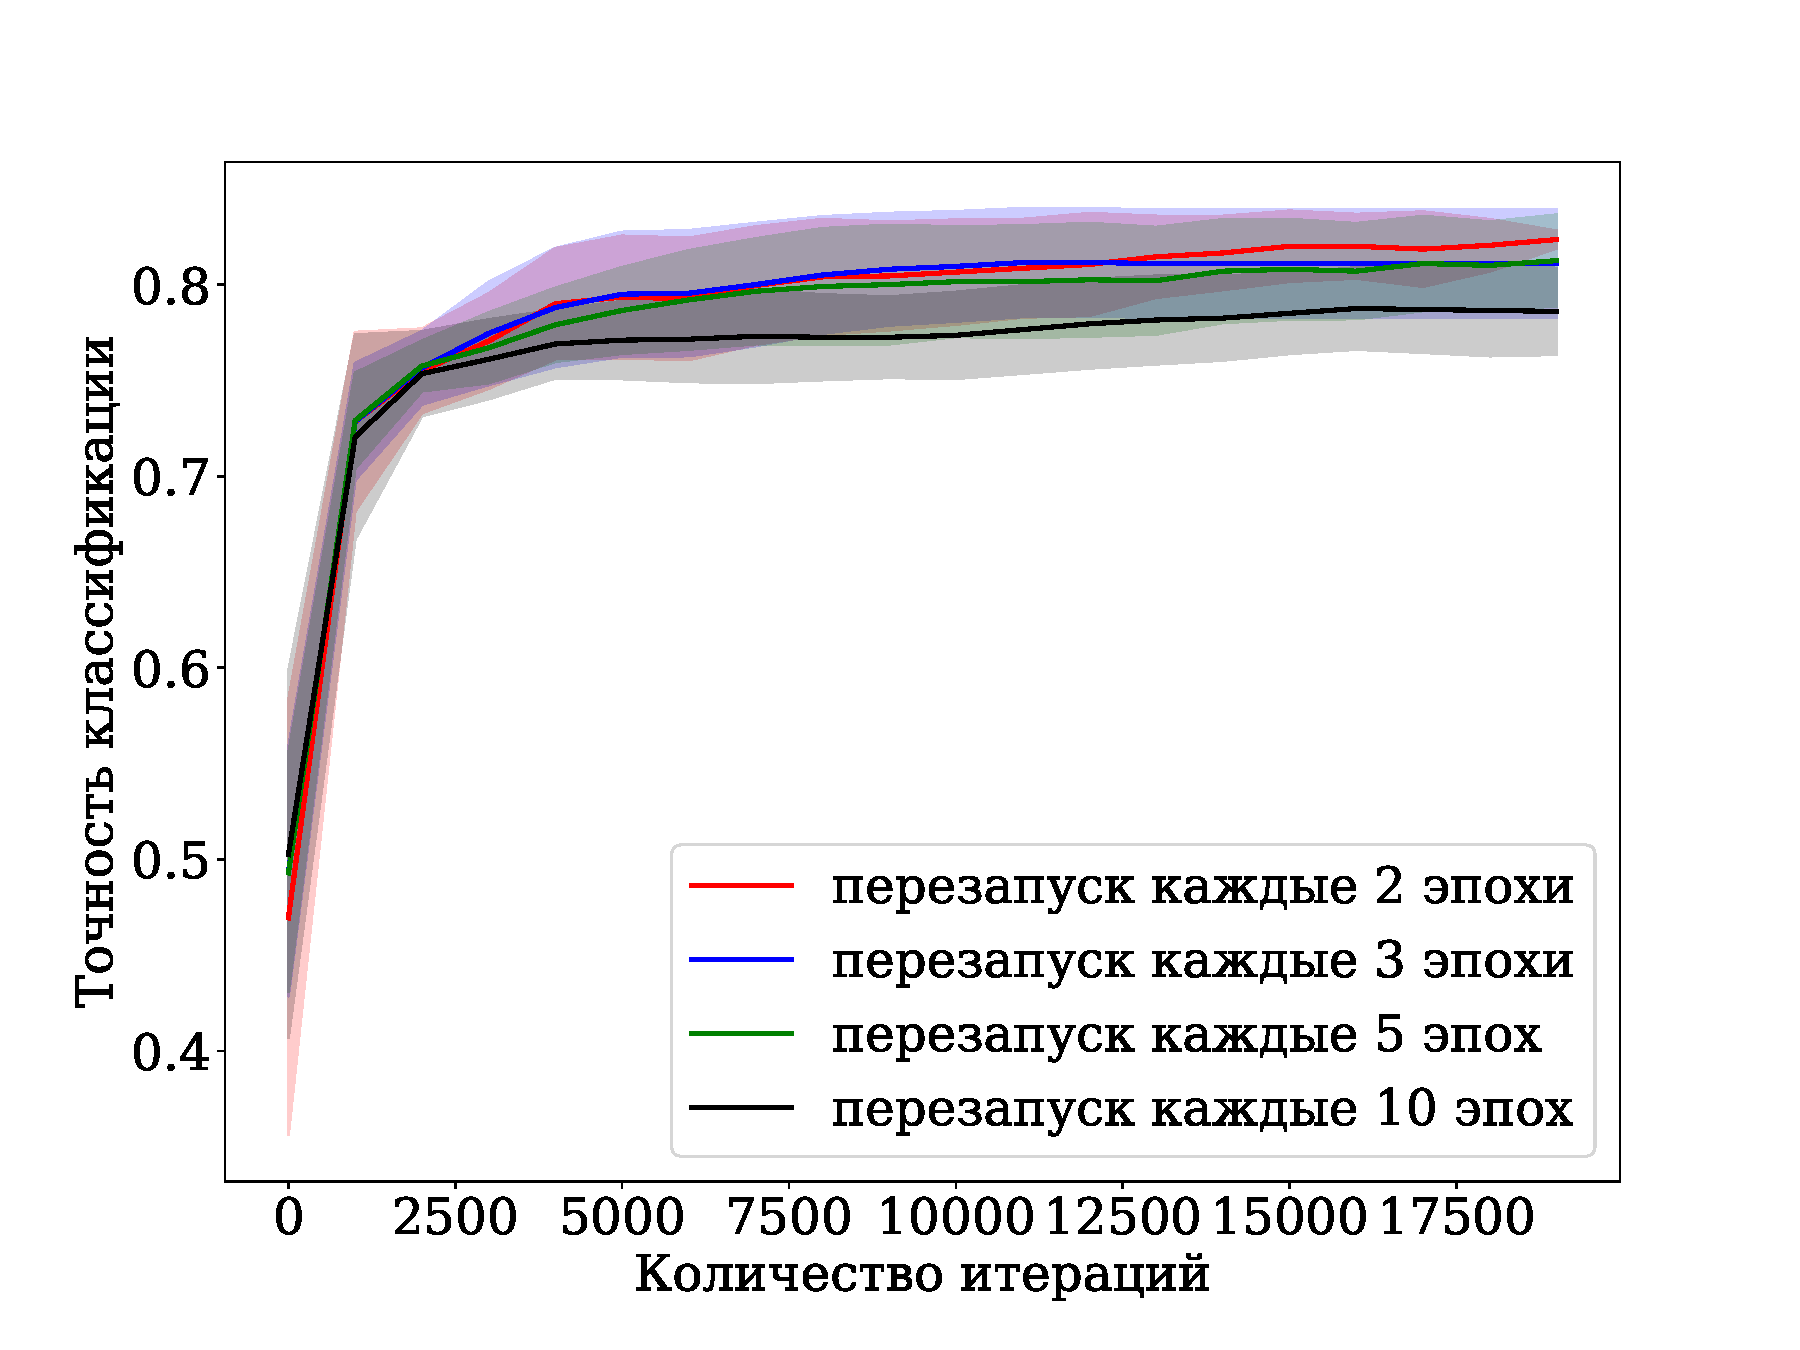
\includegraphics[width=0.6\textwidth]{linear_train_splines_every_epoch.pdf}
\caption{График зависимости точности классификации от номера итерации при различных~$n$}
\label{fig:train_splines_every_epoch}
\end{figure}

Пусть~$n$ --- число эпох между использованием сплайнов. На рис. \ref{fig:train_splines_every_epoch} показан график зависимости точности от номера итерации различных~$n$. Наилучшие результаты достигнуты при~$n=2$.

\begin{figure}[!ht]
\centering
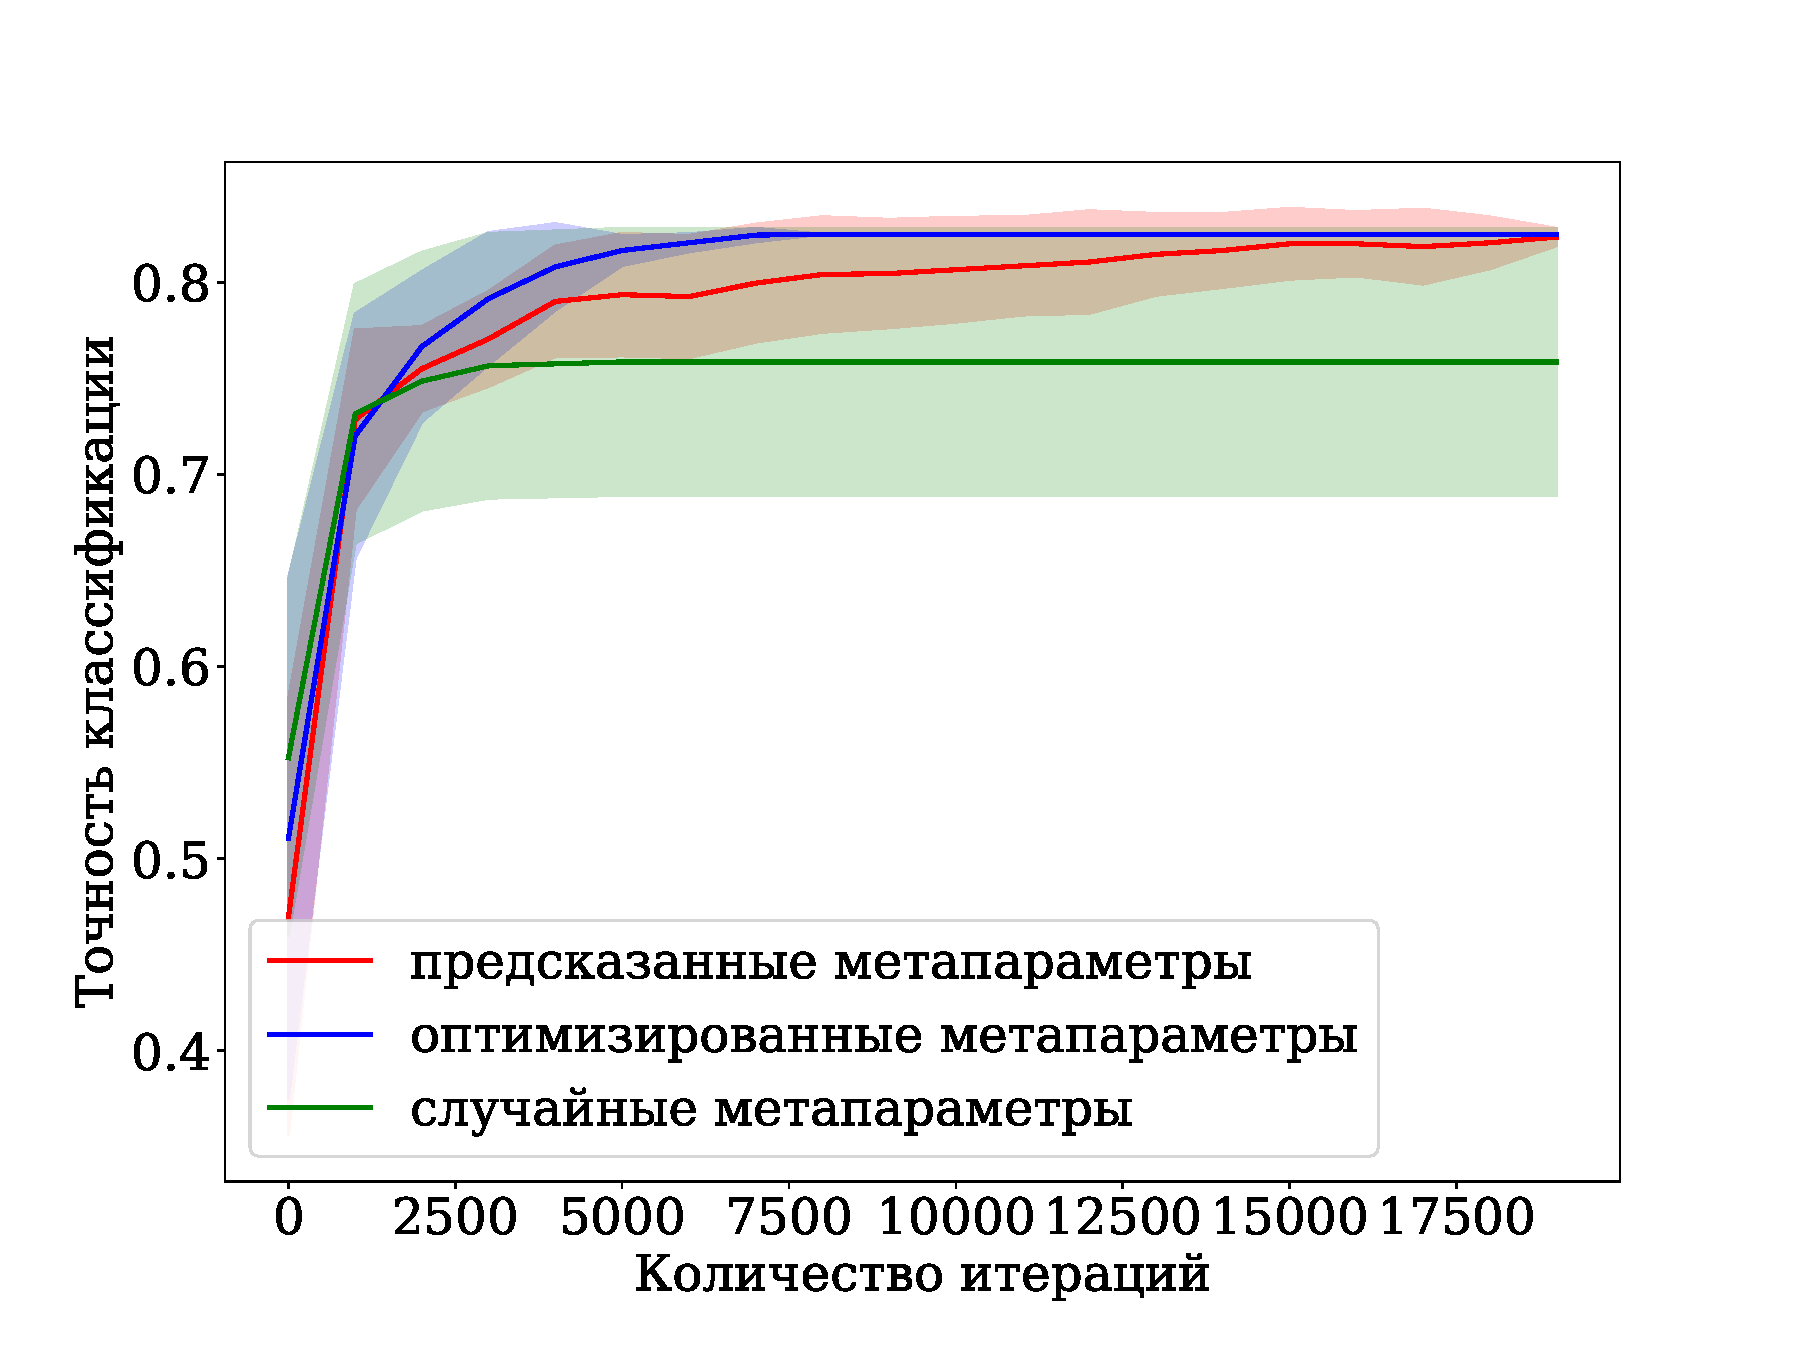
\includegraphics[width=0.6\textwidth]{acc_iter.pdf}
\caption{График зависимости точности классификации от номера итерации}
\label{fig:acc_iter}
\end{figure}

На рис. \ref{fig:acc_epoch} показан график зависимости точности от номера итерации при различных подходах к обучению модели. Наилучшие результаты достигнуты при использовании оптимизированных метапараметров, но предсказание траектории с помощью сплайнов показало результат не намного хуже предыдущего, причем с увеличением числа итераций точность этих двух методов становилась одинаковой.

\begin{figure}[!ht]
% \center{
\begin{minipage}[h]{0.5\linewidth}
\center{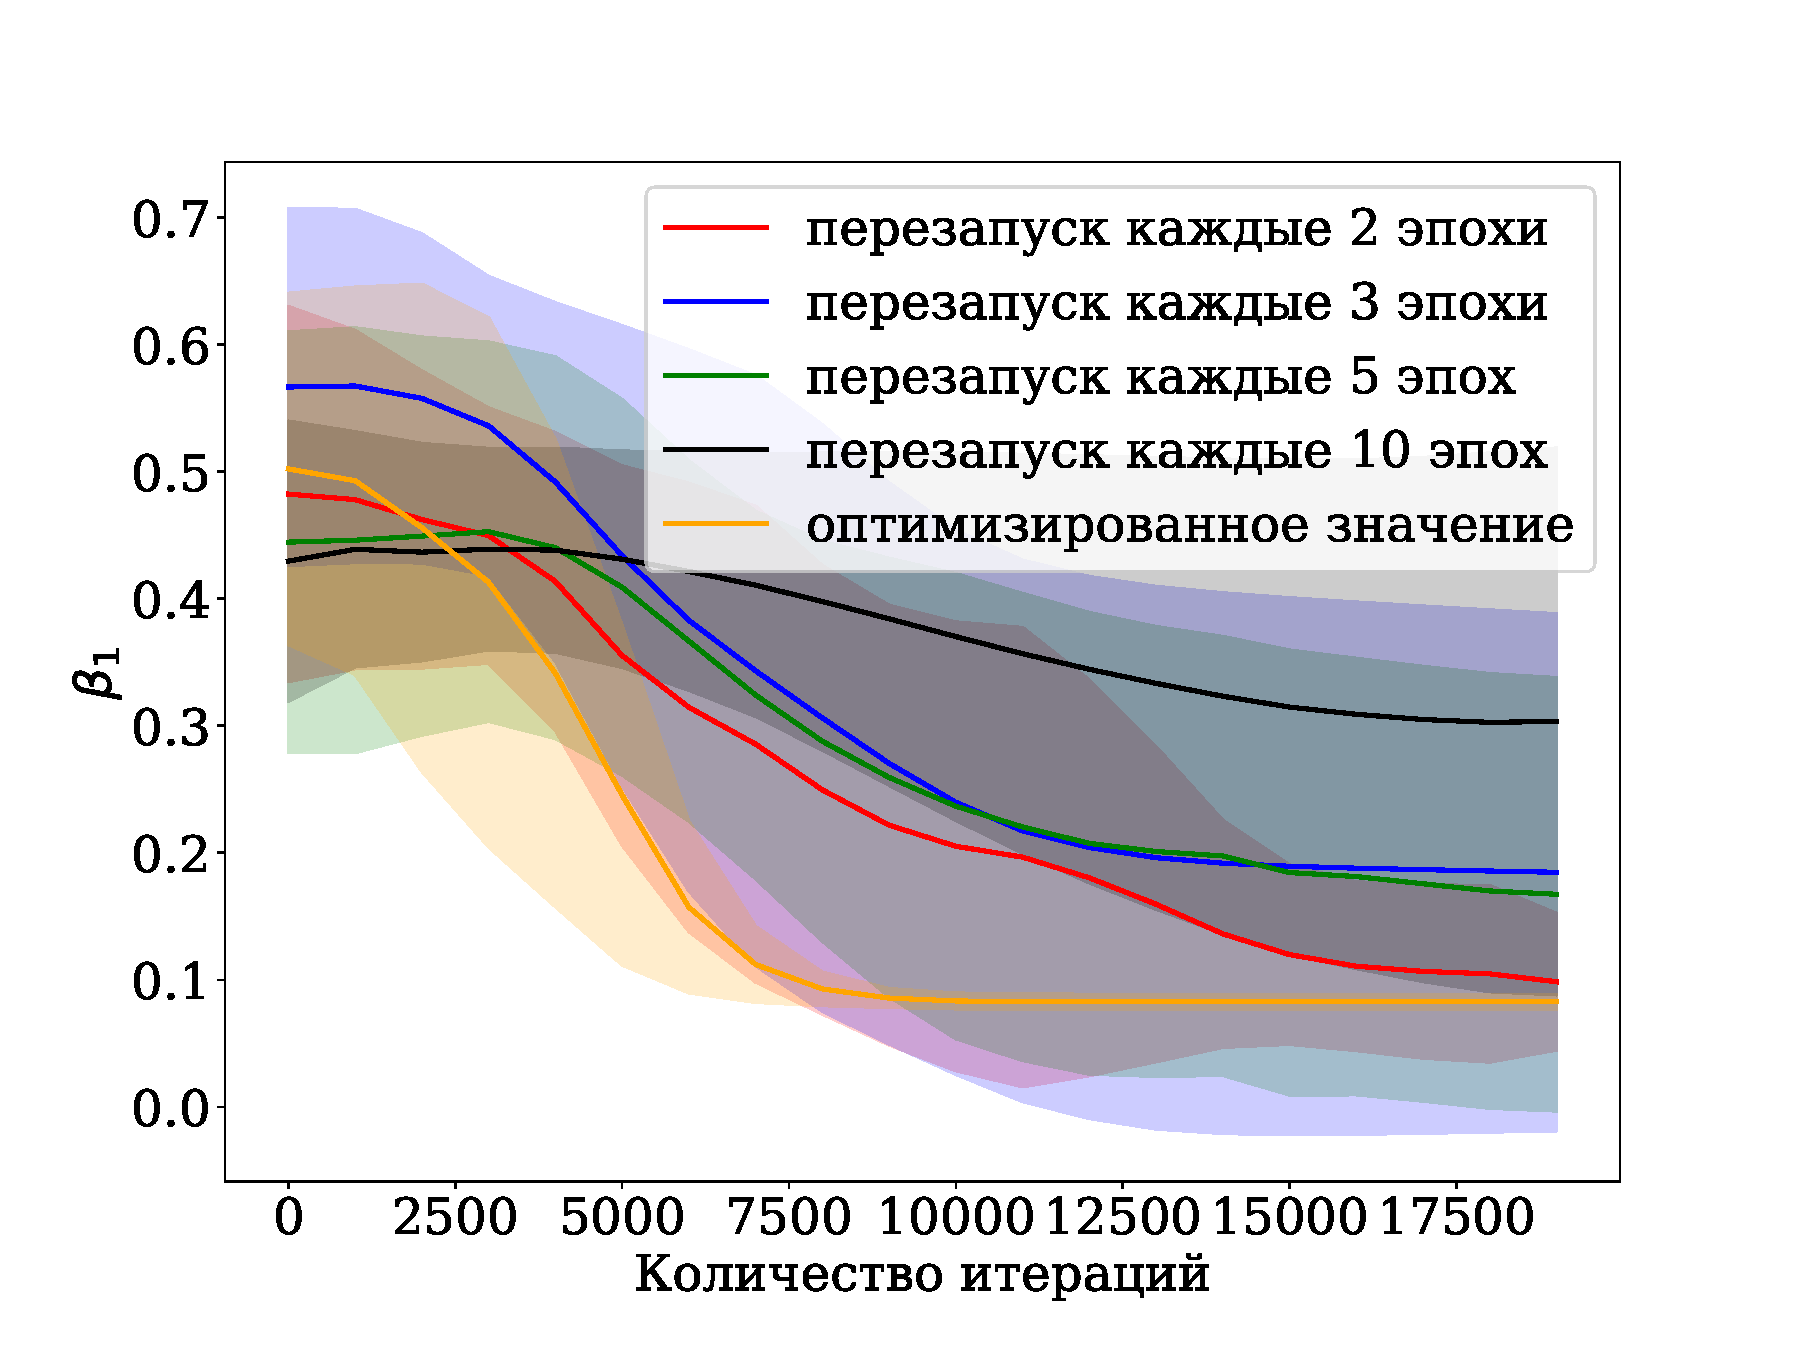
\includegraphics[width=\linewidth]{beta1_iter.pdf}\\а)}
\end{minipage}
\begin{minipage}[h]{0.5\linewidth}
\center{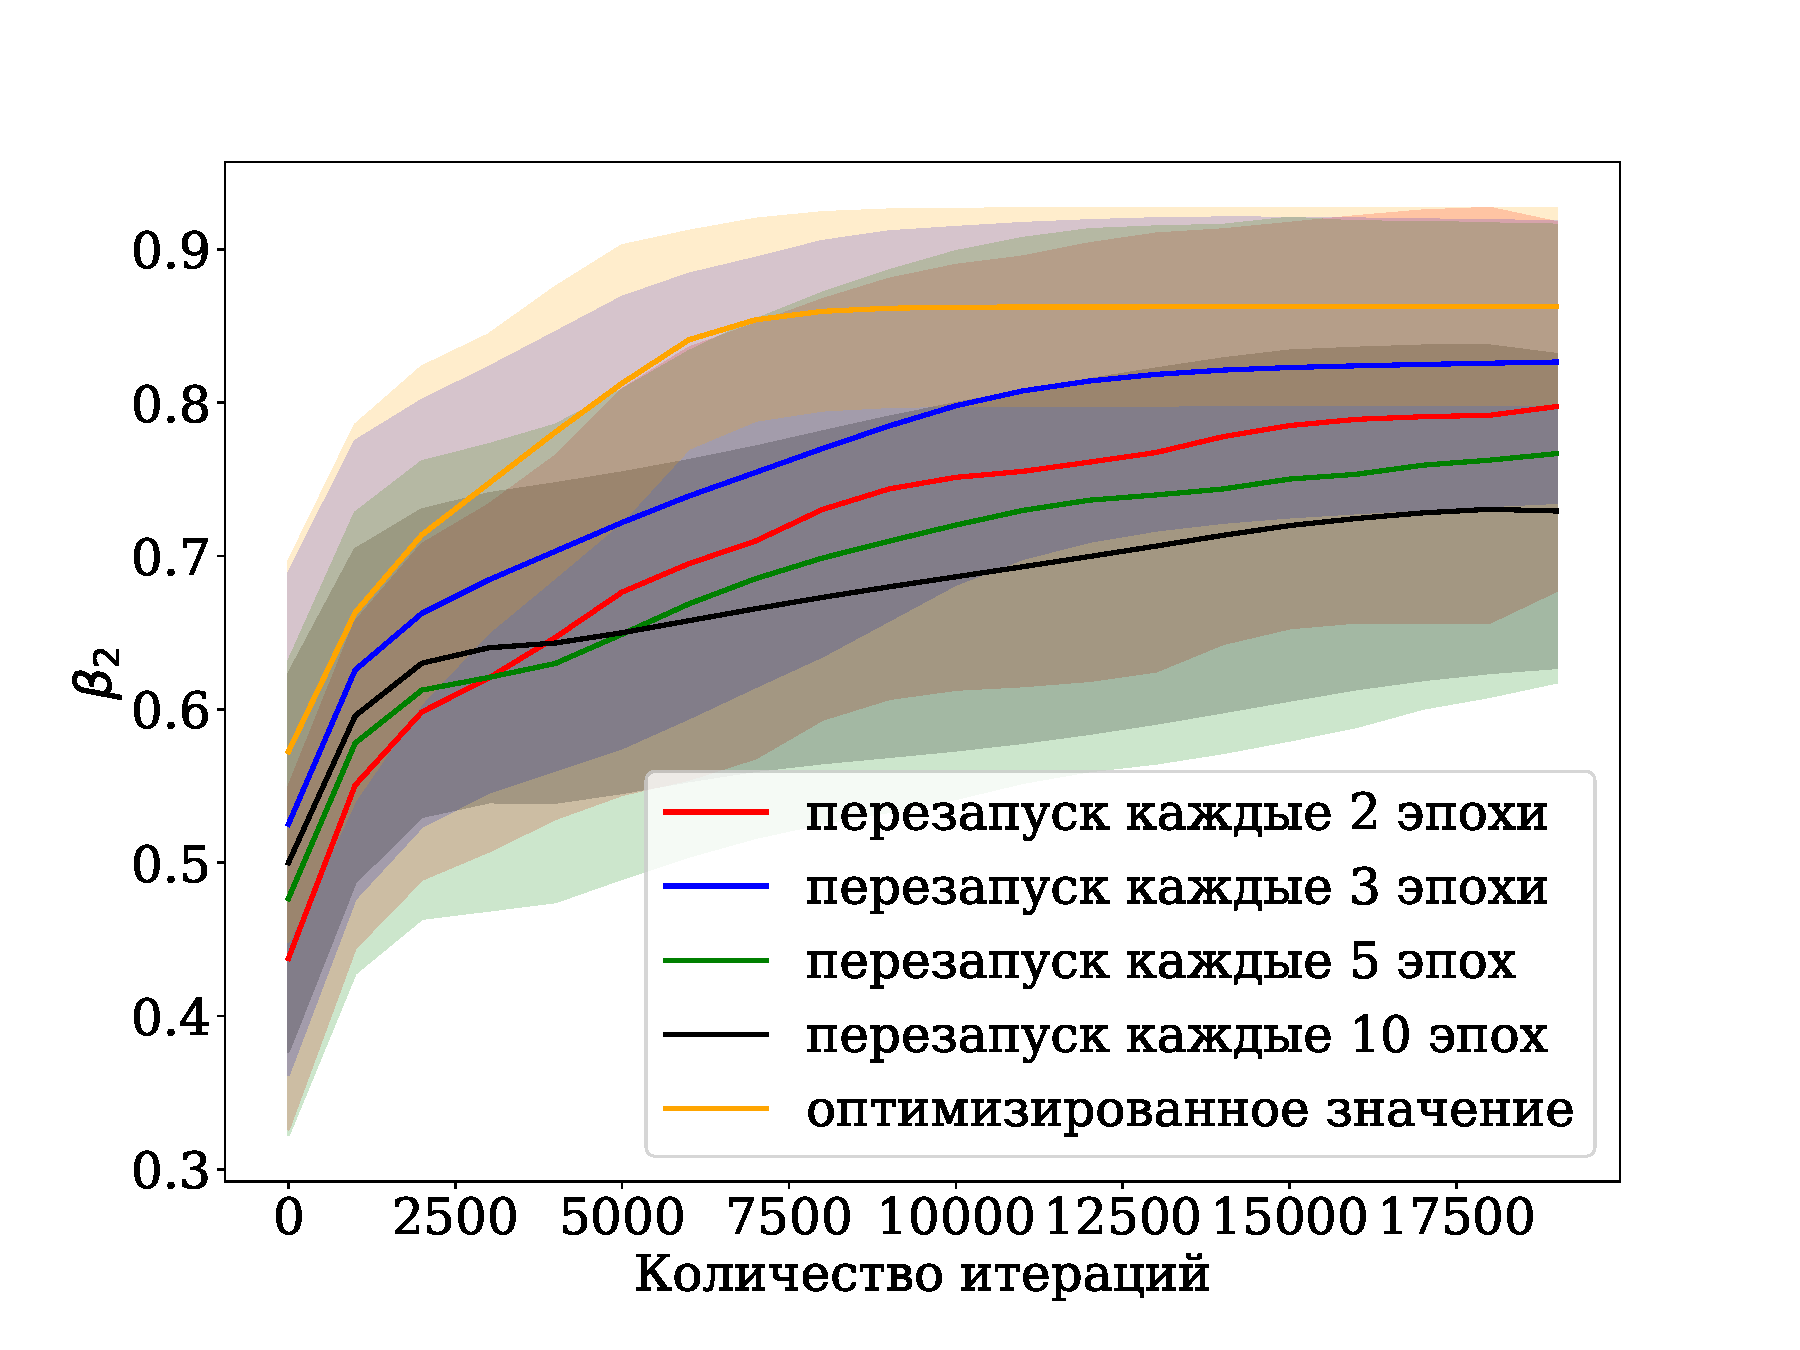
\includegraphics[width=\linewidth]{beta2_iter.pdf}\\б)}
\end{minipage}
\center{
\begin{minipage}[h]{0.5\linewidth}
\center{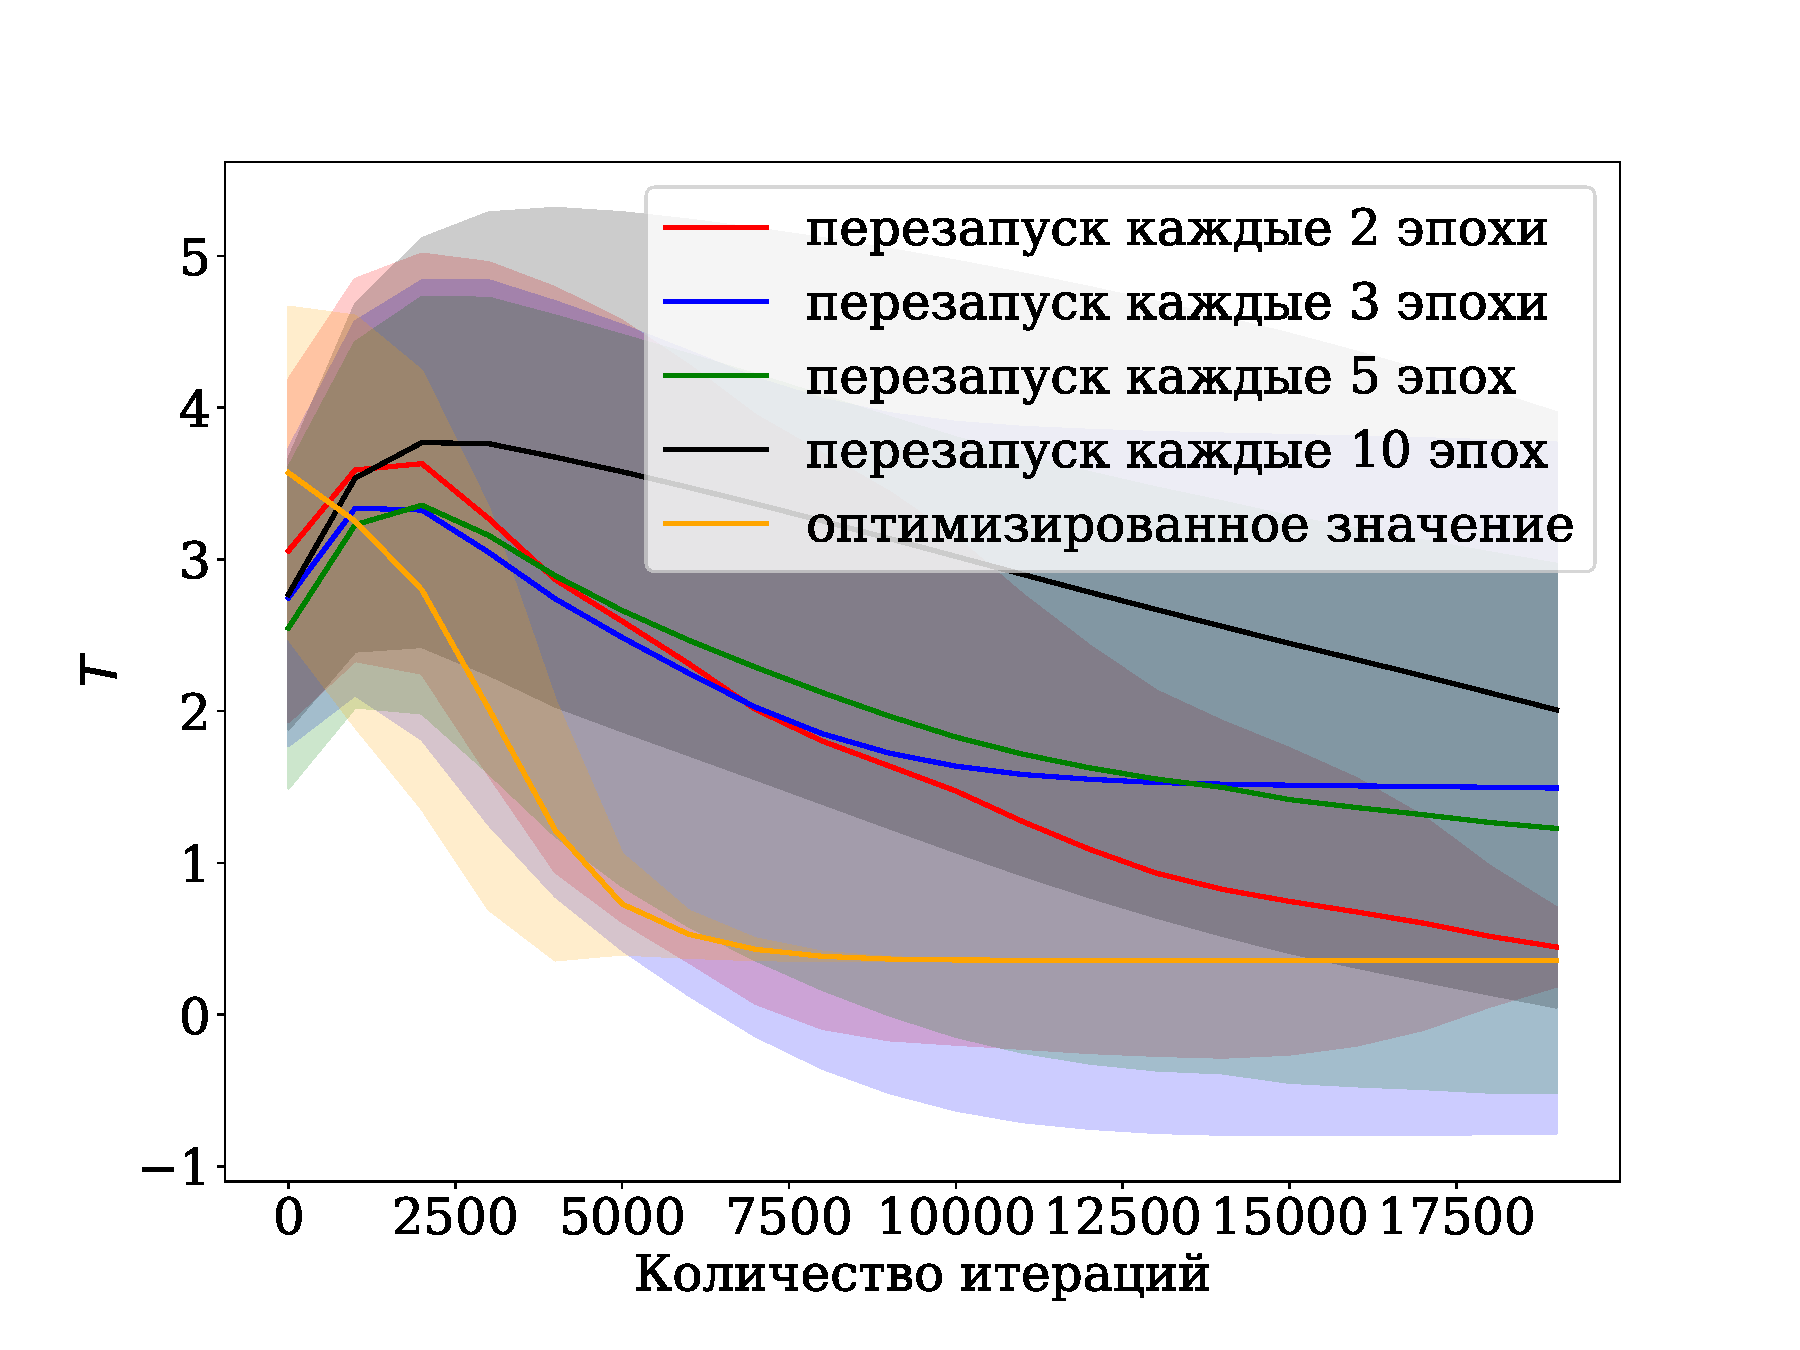
\includegraphics[width=\linewidth]{temp_iter.pdf}\\в)}
\end{minipage}}
\caption{График зависимости а)~$\lambda_1$; б)~$\lambda_2$; в) температуры от номера итерации}
\label{fig:meta_iter}
\end{figure}

% \begin{figure}[!ht]
%     \centering
%     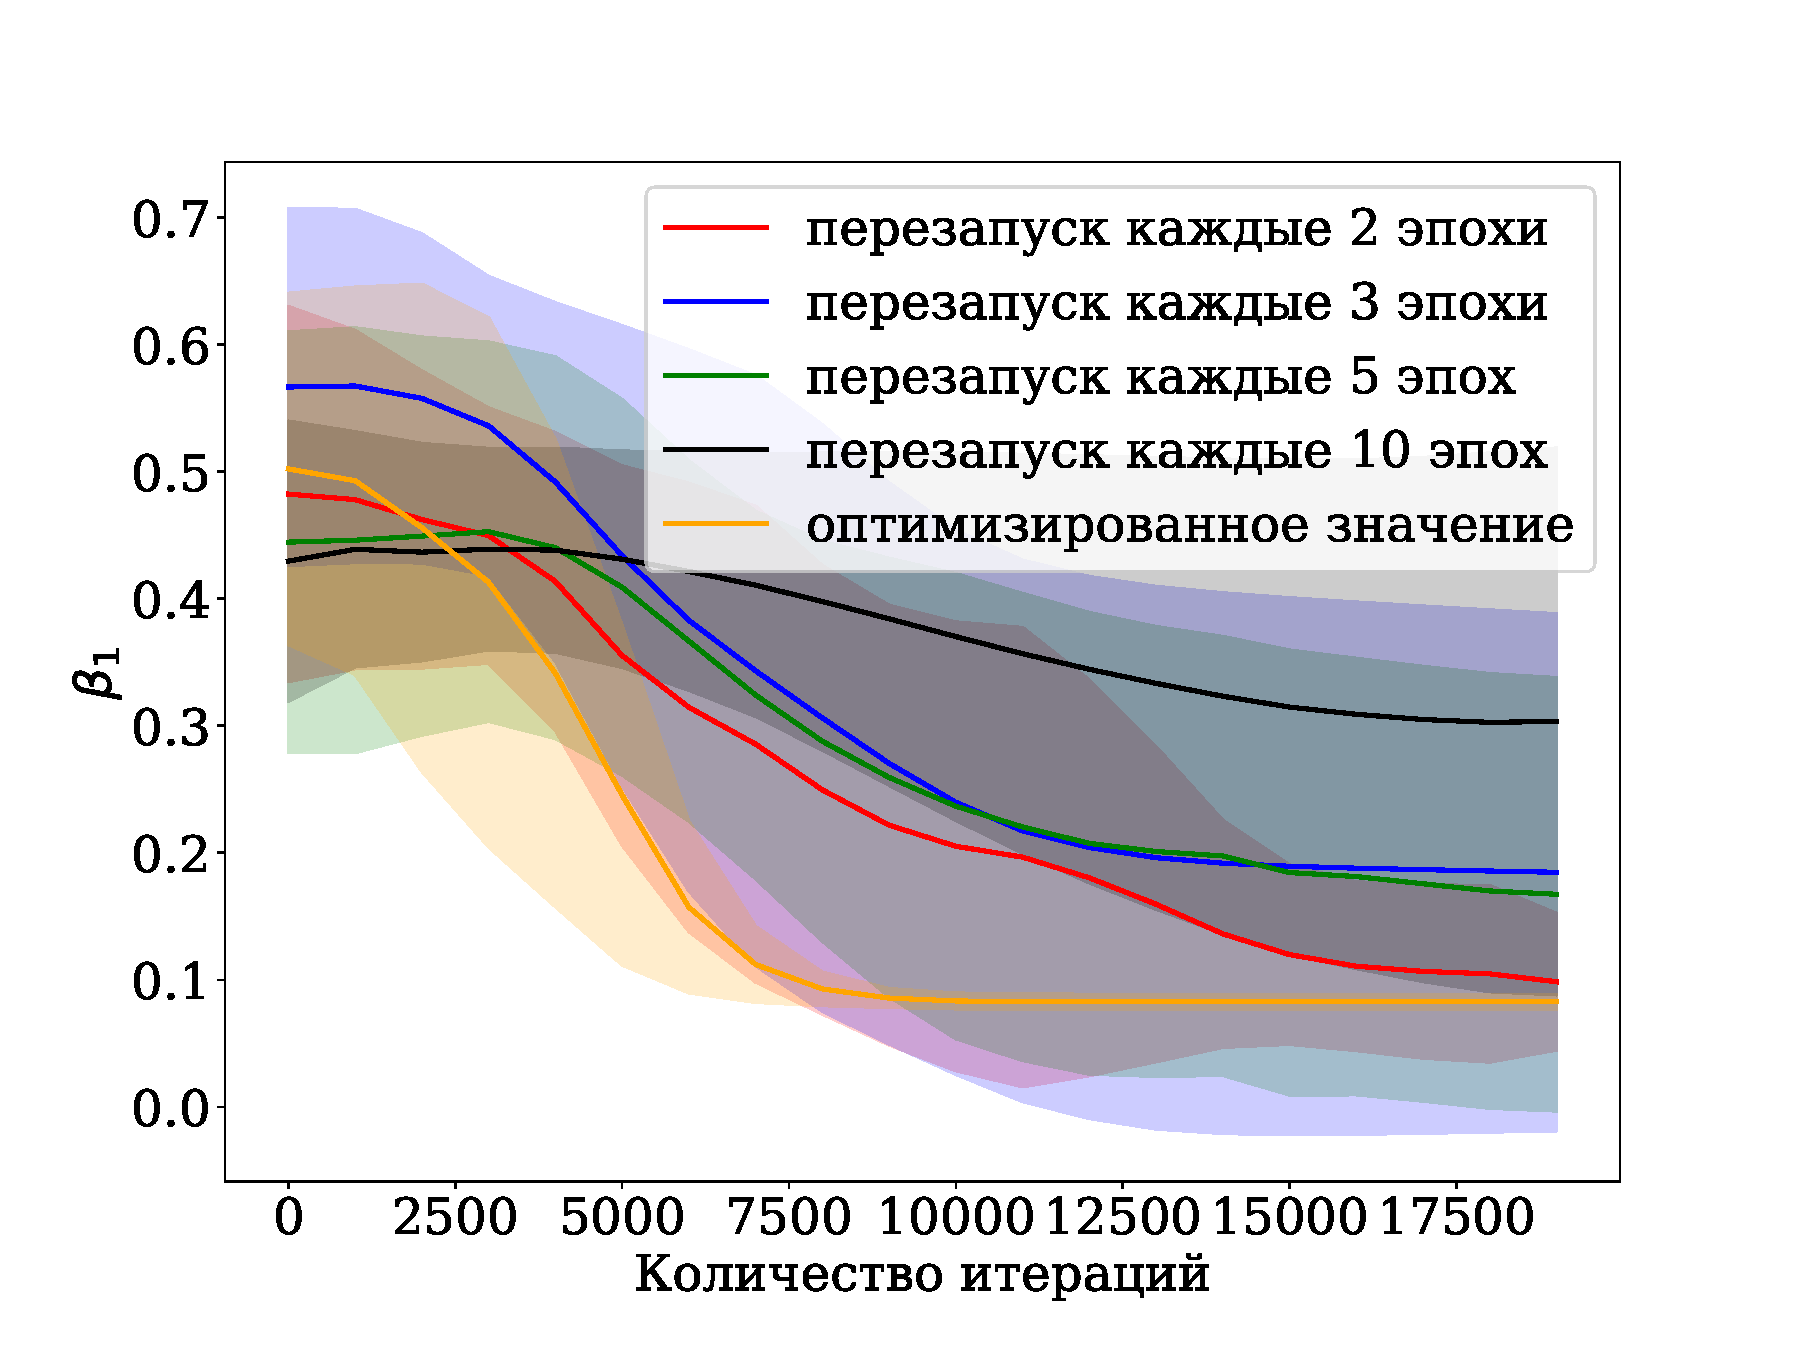
\includegraphics[width=0.6\textwidth]{beta1_iter.pdf}
%     \caption{График зависимости значения $\lambda_1$ от номера итерации}
%     \label{fig:beta1_it}
% \end{figure}

% \begin{figure}[!ht]
%     \centering
%     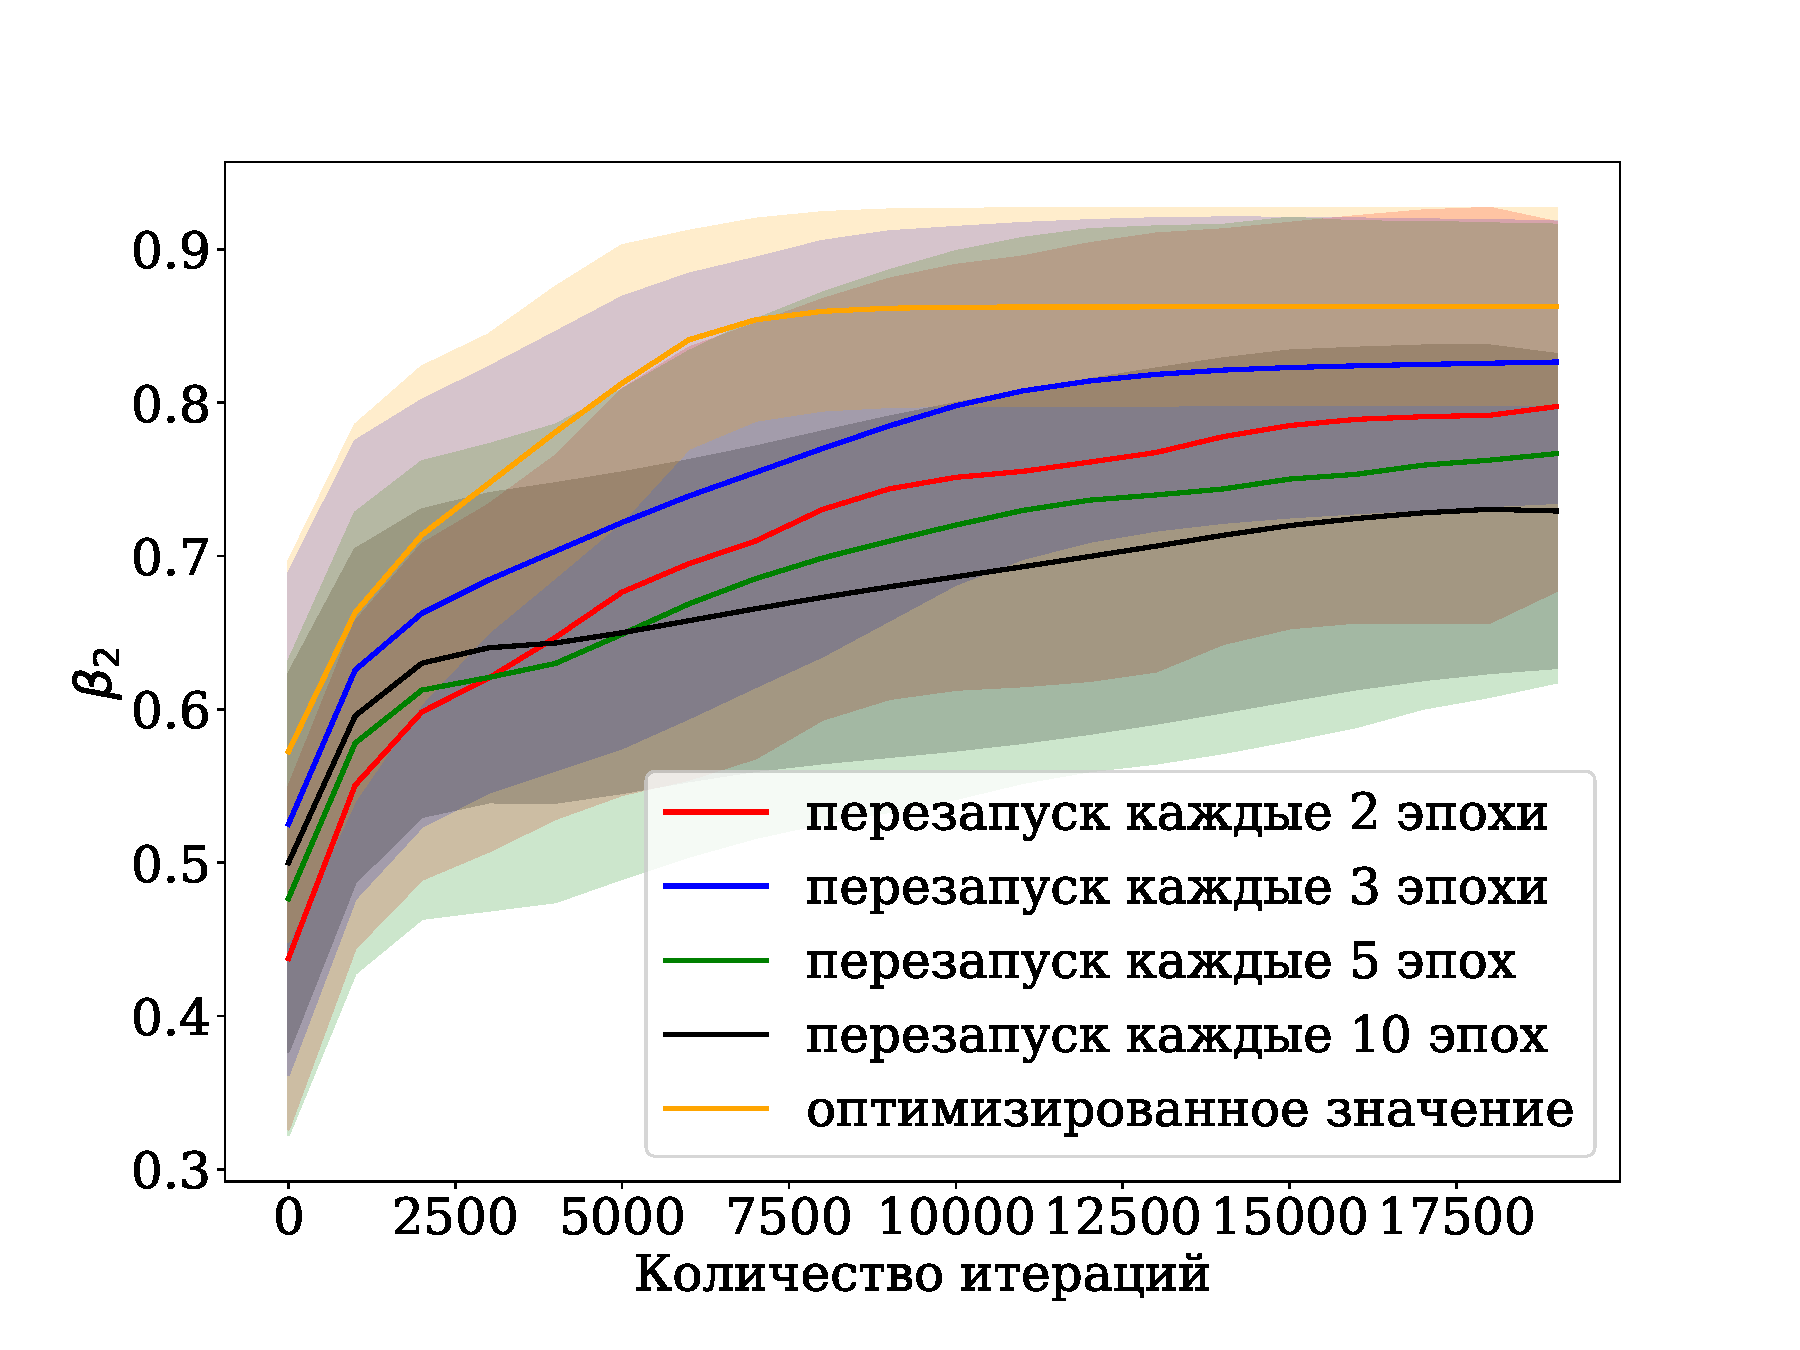
\includegraphics[width=0.6\textwidth]{beta2_iter.pdf}
%     \caption{График зависимости значения $\lambda_2$ от номера итерации}
%     \label{fig:beta2_it}
% \end{figure}

% \begin{figure}[!ht]
%     \centering
%     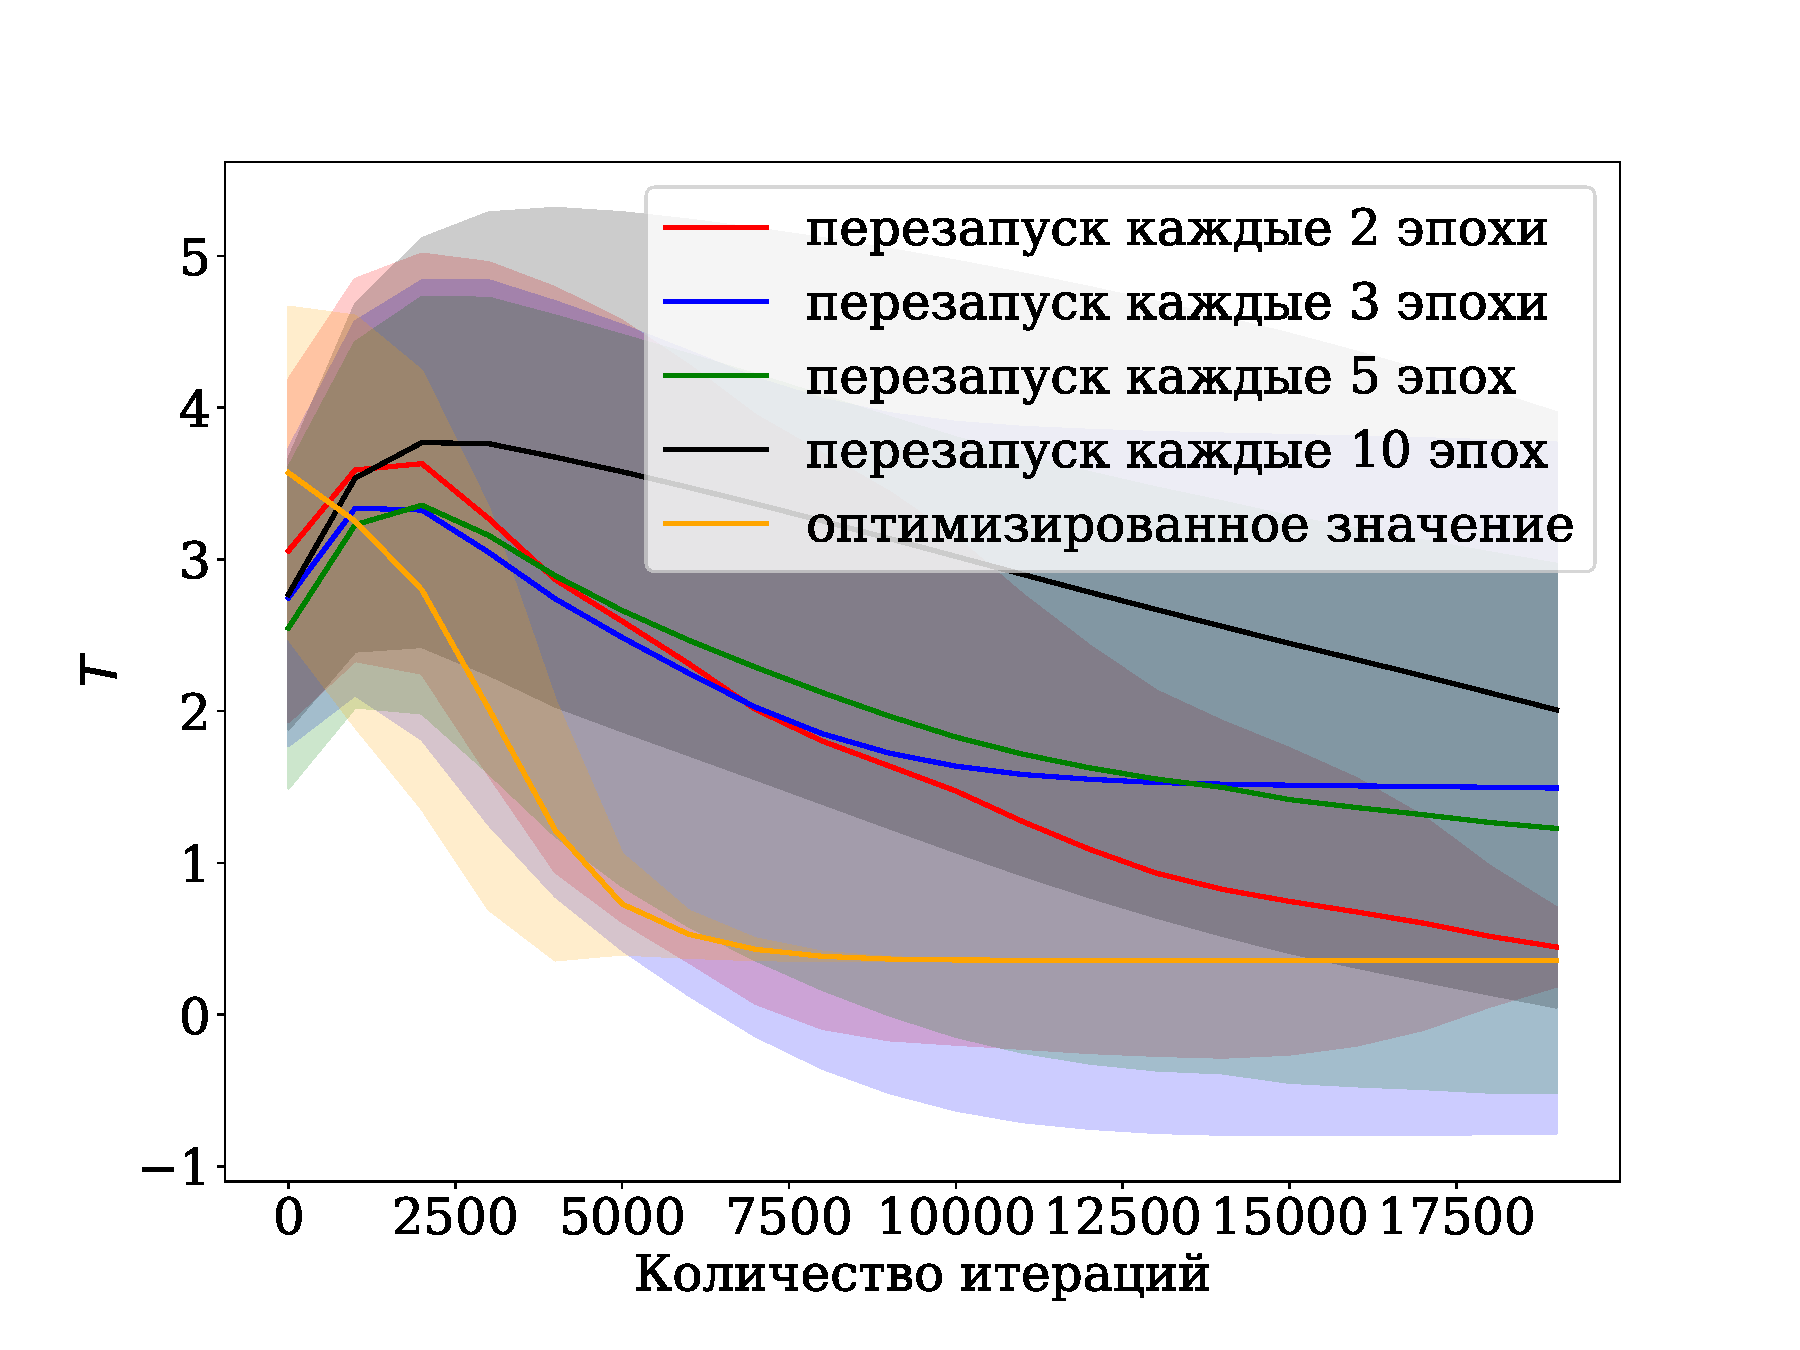
\includegraphics[width=0.6\textwidth]{temp_iter.pdf}
%     \caption{График зависимости значения $T$ от номера итерации}
%     \label{fig:temp_it}
% \end{figure}

% На рис. \ref{fig:beta1_it}, \ref{fig:beta2_it} и \ref{fig:temp_it} показаны графики обновления метапараметров $\lambda_1$, $\lambda_2$ и $T$. Из графика видно, что при $n=2$, предсказанная траектория наиболее близка к траектории, полученной с помощью только градиентных методов.

\subsection{Эксперимент на выборке CIFAR-10}
В эксперименте используется выборка CIFAR-10, которая состоит из~$60000$ цветных изображений размера~$32 \times 32$ пикселя, разделенных на 10 непересекающихся классов. К каждому классу относится~$6000$ изображений. Выборка делится на обучающую ($50000$ изображений) и тестовую ($10000$ изображений) подвыборки. В тестовой выборке содержится~$1000$ изображений каждого класса.

Внешним критерием качества модели является точность~$\eqref{eq:accuracy}$. В качестве моделей-учителей рассматриваются модели из~\cite{conf/cvpr/PassalisTT20}, а именно, ResNet-18 и сверточная нейросеть с тремя сверточными слоями и двумя слоями полносвязной нейросети.

Проведено сравнение среднего качества обучения модели-ученика без дистилляции после~$5$ запусков, с дистилляцией с моделью-учителем ResNet и сверточной нейросетью после 20 запусков. Значение коэффициента~$\lambda$ лежит в пределах от 0 до 1, значение температуры~---~от 0.1 до 10.

\begin{figure}[!ht]
\centering
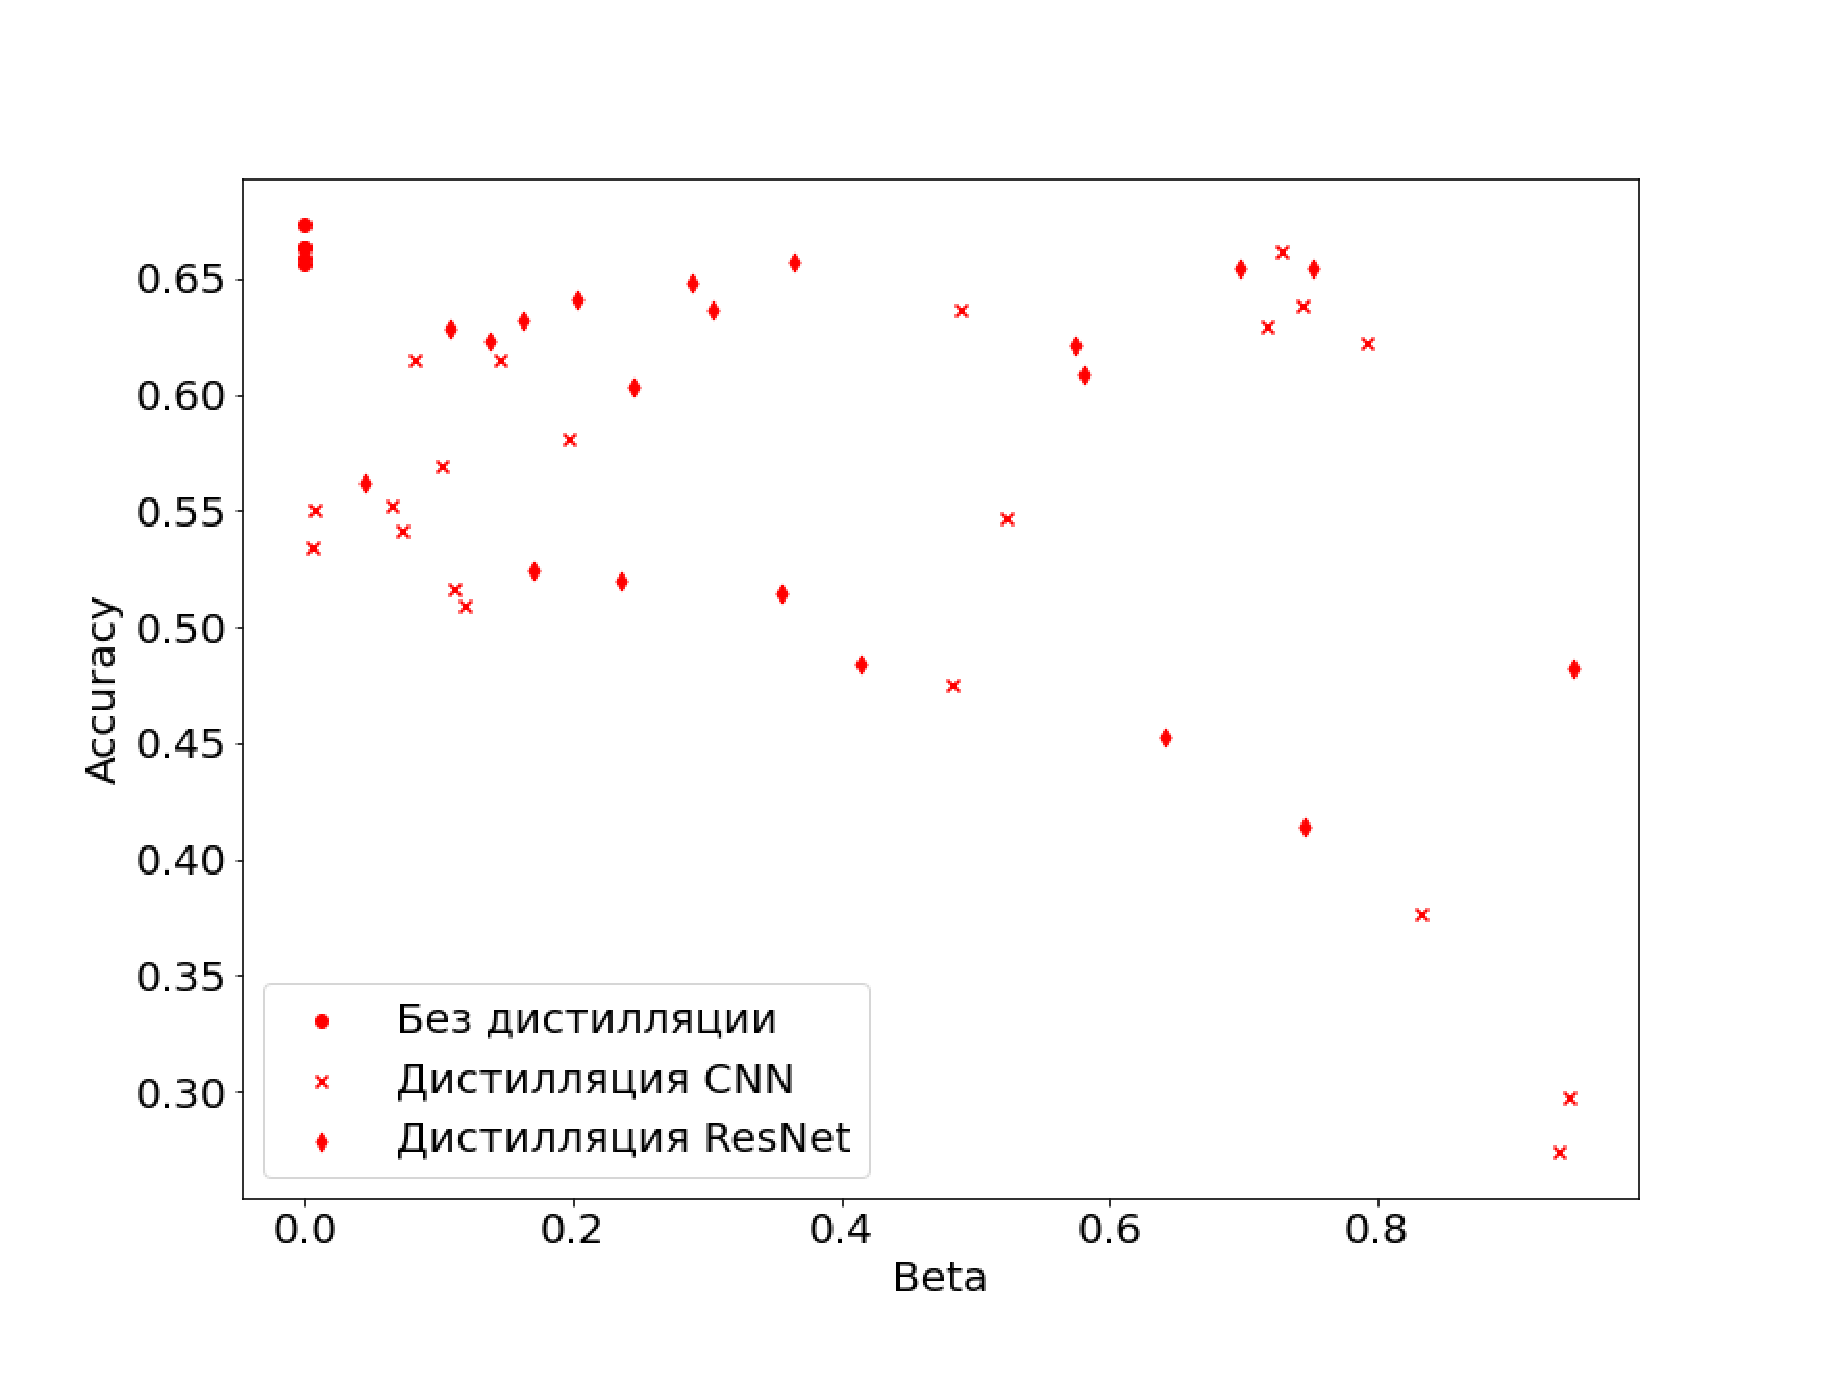
\includegraphics[width=0.5\textwidth]{scatter_beta_acc.eps}
\caption{График зависимости точности от~$\lambda$}
\label{fig:beta_acc}
\end{figure}

\begin{figure}[!ht]
\centering
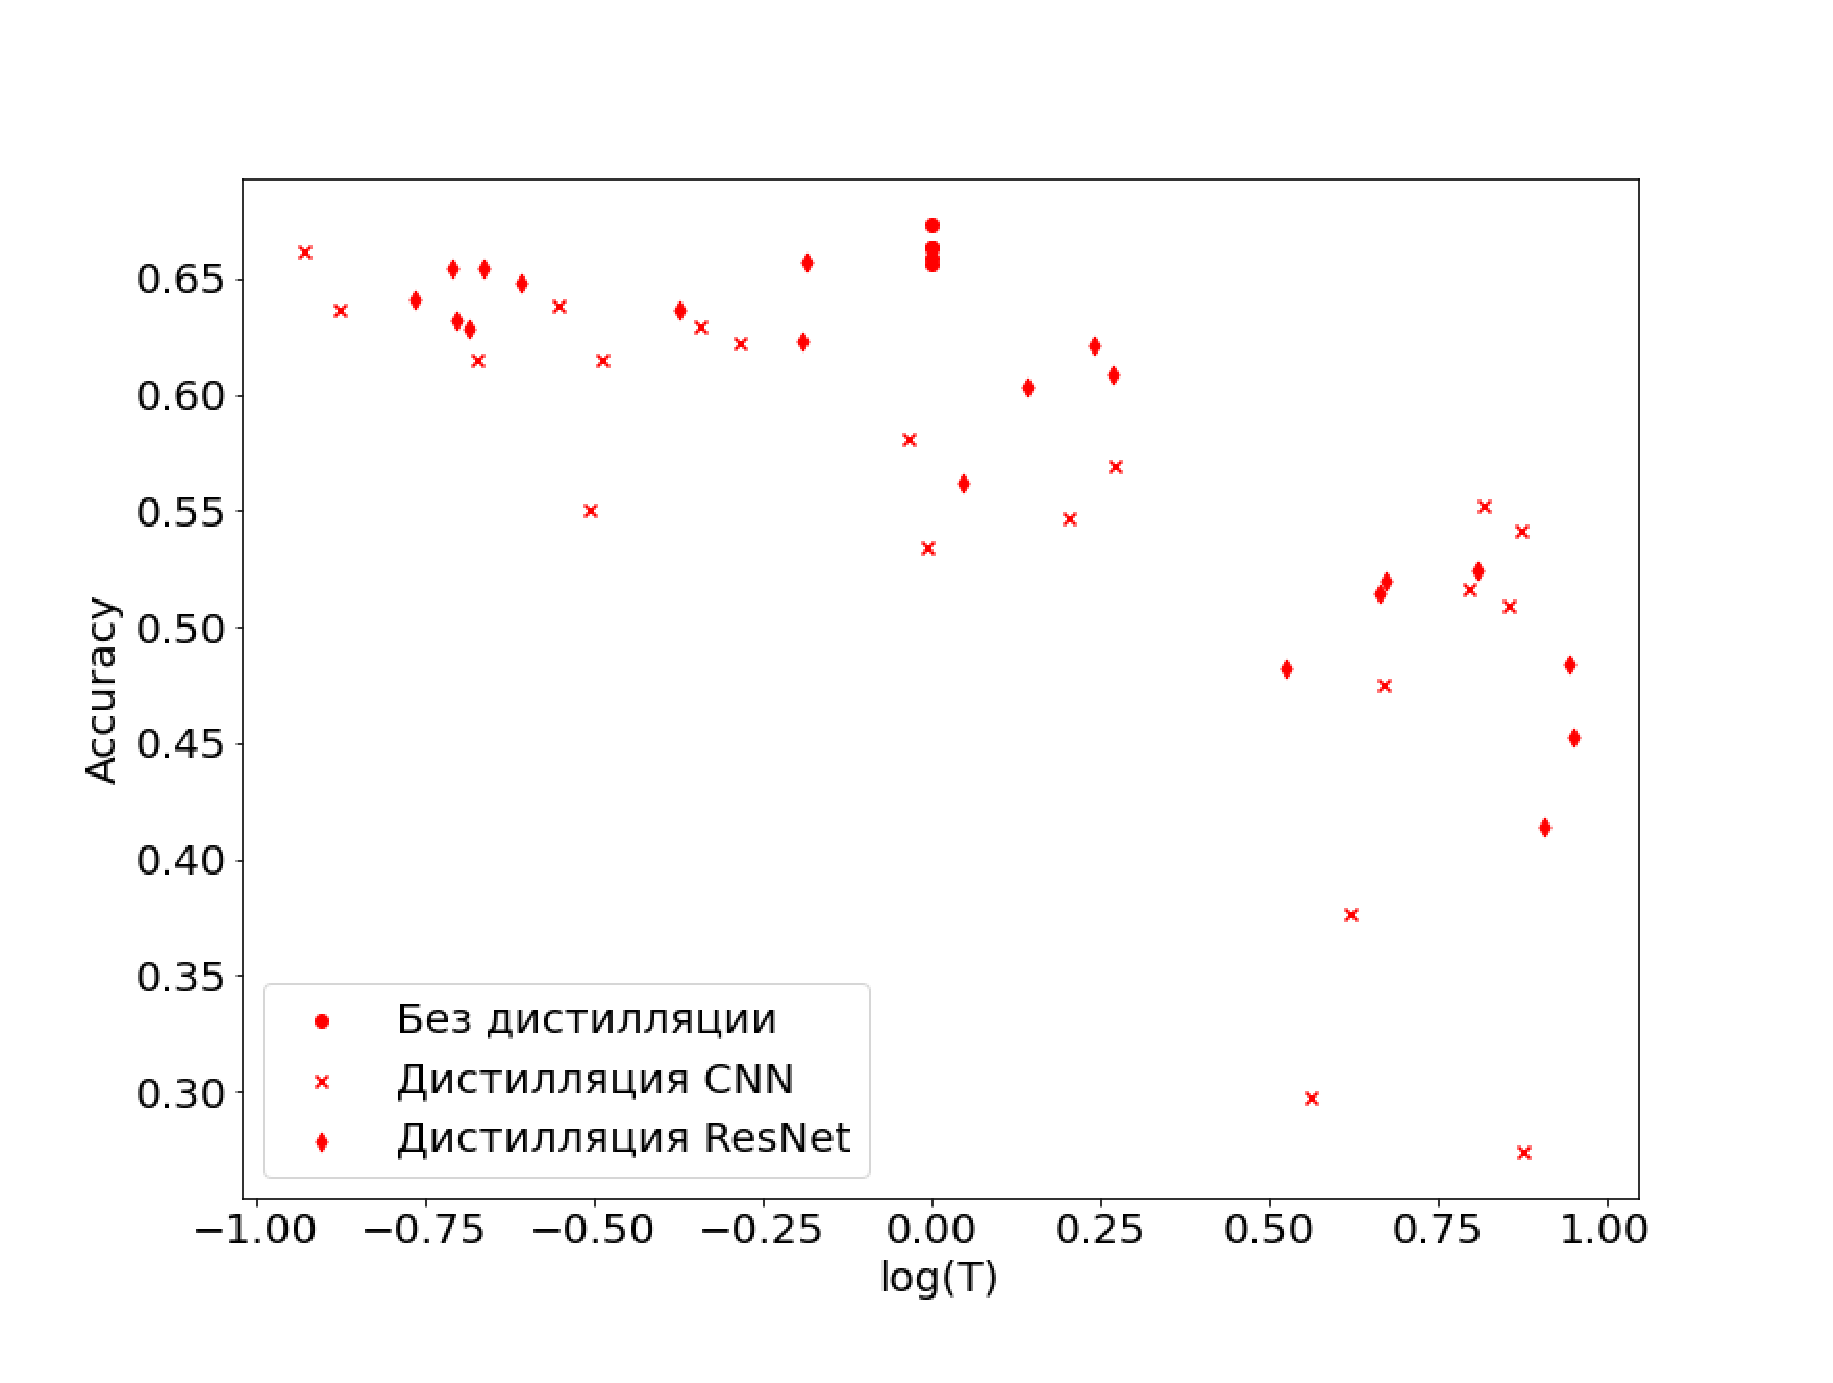
\includegraphics[width=0.5\textwidth]{scatter_temp_acc.eps}
\caption{График зависимости точности от температуры}
\label{fig:temp_acc}
\end{figure}

\begin{figure}[!ht]
\centering
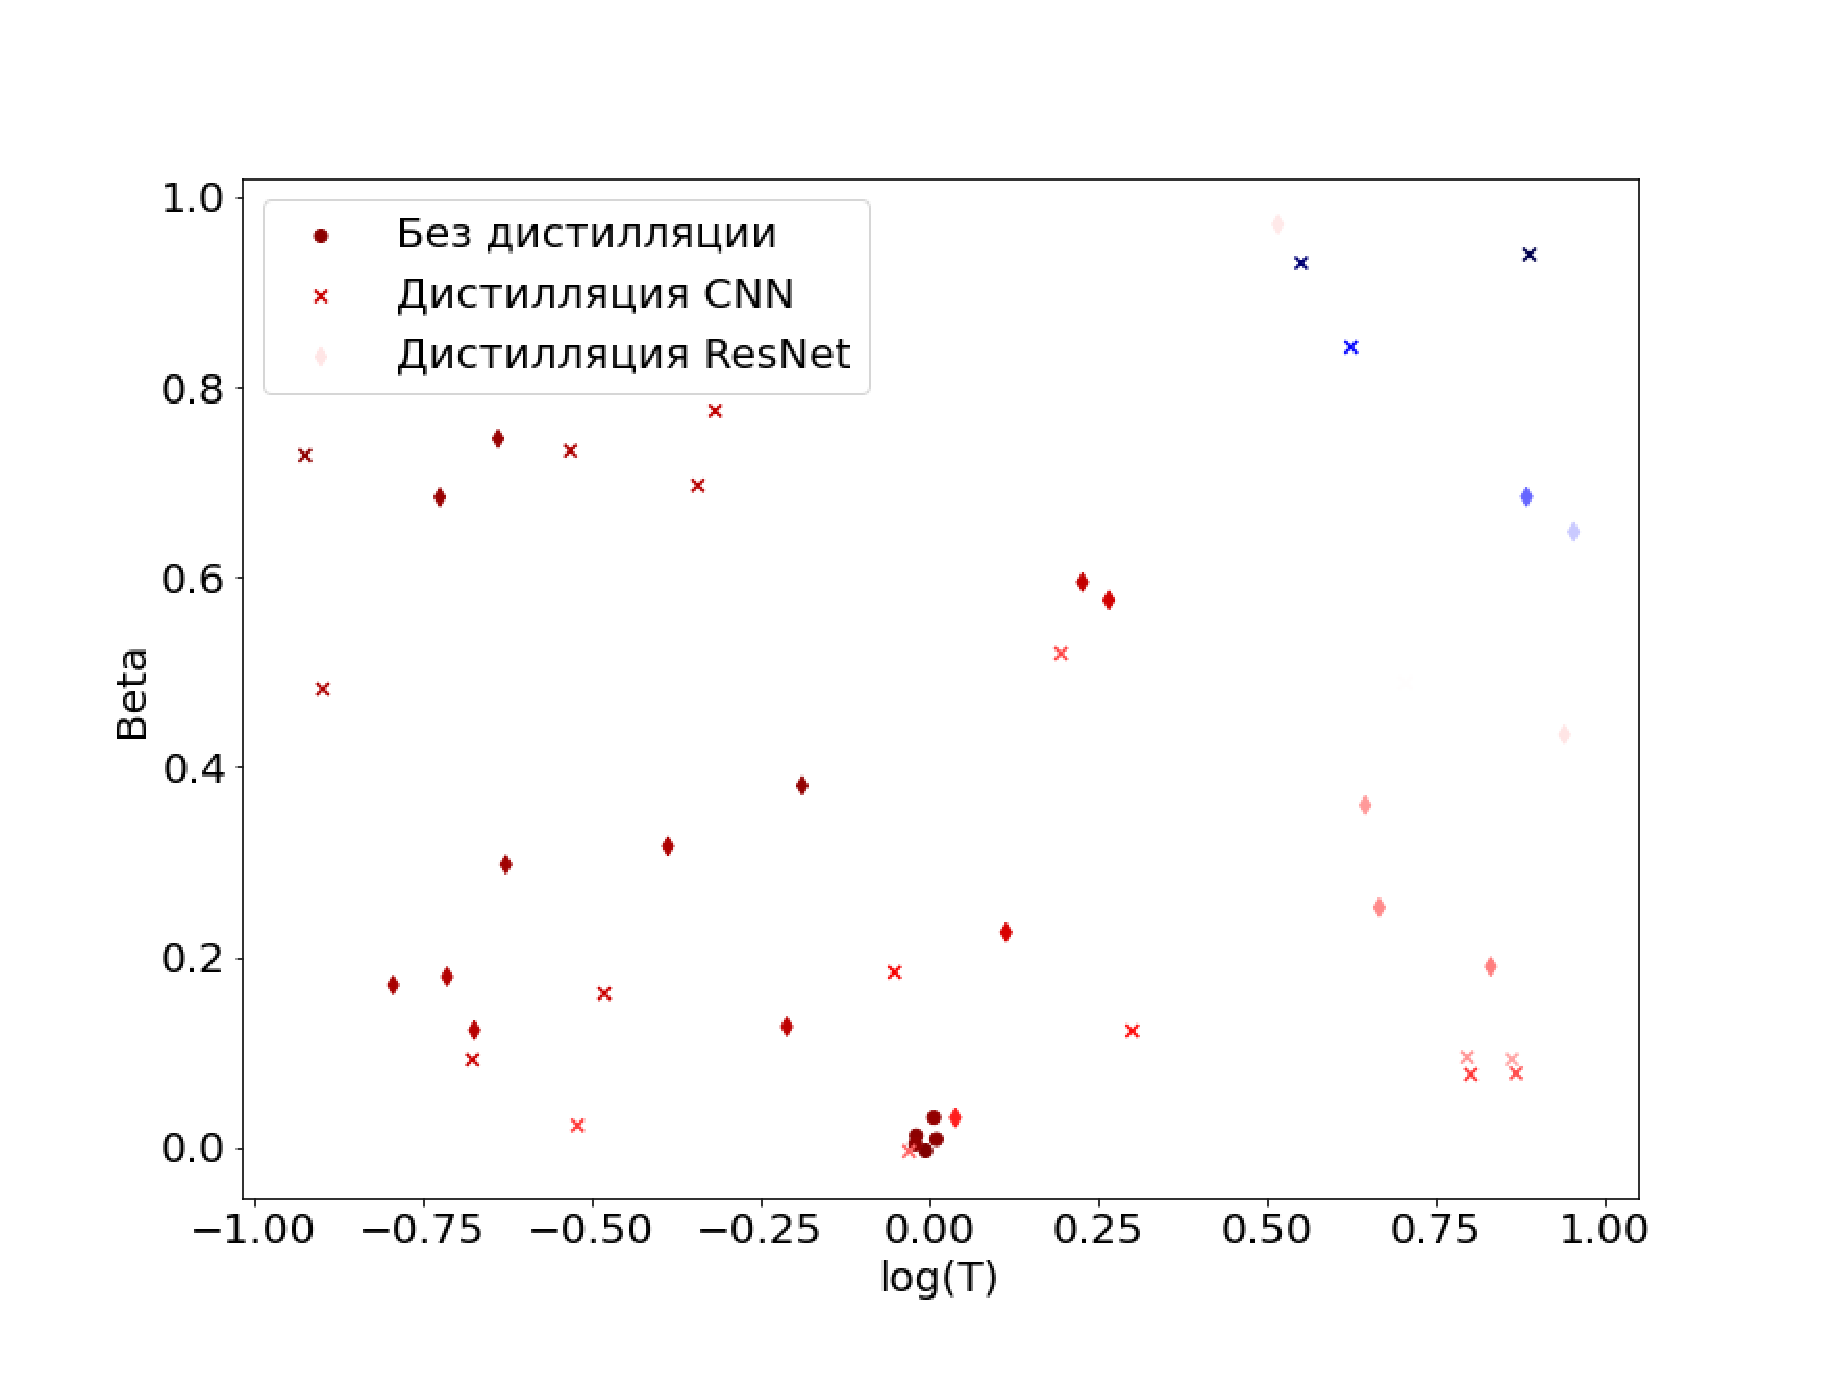
\includegraphics[width=0.5\textwidth]{scatter_temp_beta.eps}
\caption{График зависимости~$\lambda$ от температуры с выделенной цветом~$\text{accuracy}$}
\label{fig:temp_beta}
\end{figure}

На~рис. \ref{fig:beta_acc} изображена зависимость точности от величины коэффициента~$\lambda$. Различные точки отвечают за точность модели без дистилляции, с дистилляцией ResNet и CNN. Можно заметить, что с уменьшением значения коэффициента~$\lambda$ значение точности увеличивается.

На~рис. \ref{fig:temp_acc} изображена зависимость точности от~$T$. Для изображения значений температуры используется логарифмическая шкала. По графику видно, что значение температуры уменьшается при увеличении логарифма температуры, но при значениях логарифма от 0.5 до 1 наблюдается резкое уменьшение точности.

На~рис. \ref{fig:temp_beta} изображена зависимость~$\lambda$ от величины~$T$ с выделенной цветом~$\text{accuracy}$. Заметим, что точки с большим значением точности в основном расположены в правом нижнем углу графика, а именно, при значениях~$\lambda$ от 0 до 0.5 и значениях~$\log(T)$ от -1 до 0. Наоборот, точки с низким значением точности, расположены в правом верхнем углу графика.

\begin{figure}[!ht]
\centering
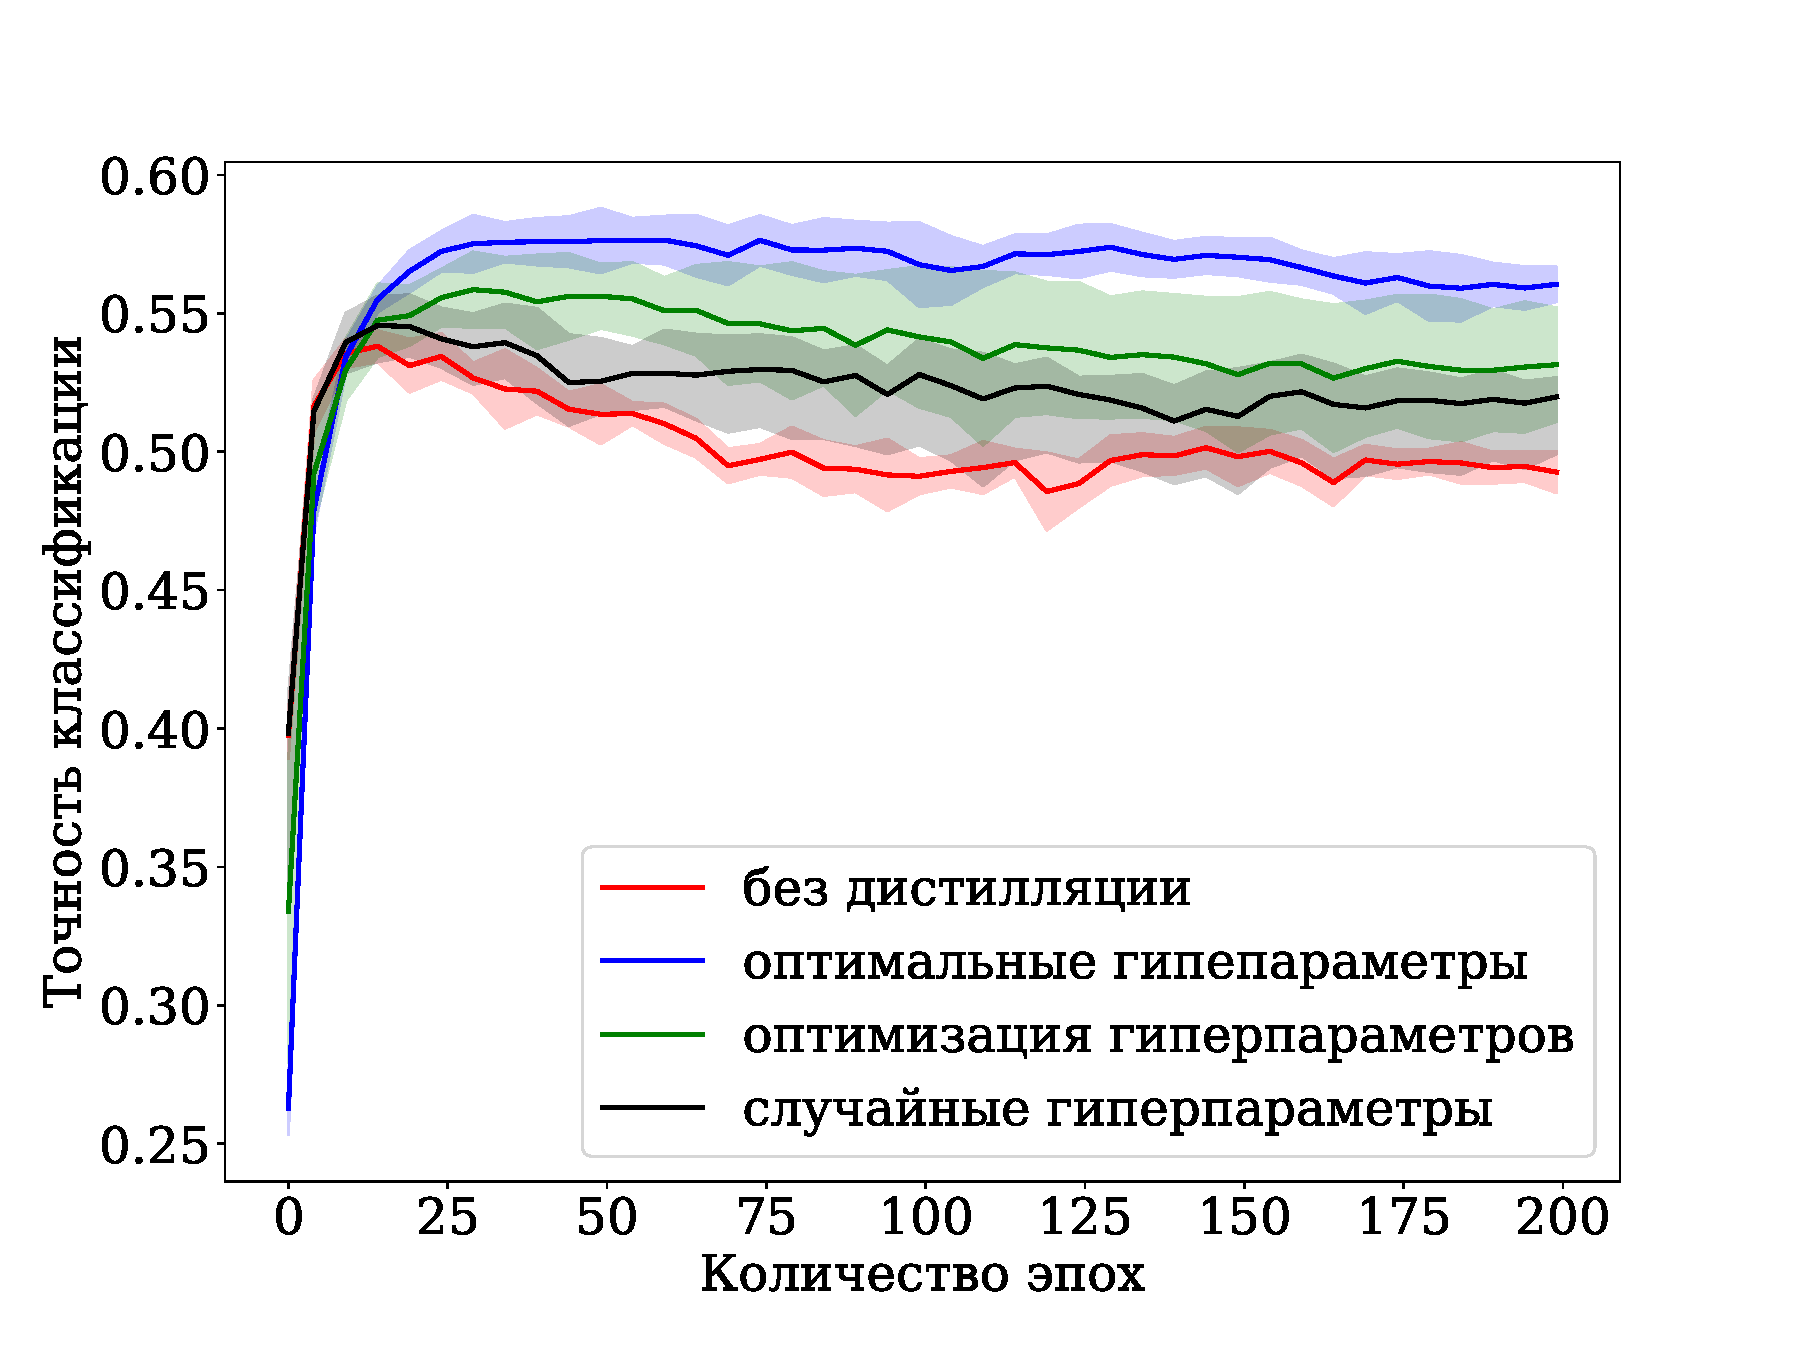
\includegraphics[width=0.5\textwidth]{slides/acc.pdf}
\caption{График зависимости точности от числа эпох}
\label{fig:acc_epoch}
\end{figure}

На~рис. \ref{fig:acc_epoch} изображена зависимость точности от числа эпох для обучения модели-ученика без дистилляции, обучения с дистилляцией и случайными метапараметрами, обучения с дистилляцией и оптимизацией метапараметров, а также обучения с дистилляцией и оптимальными метапараметрами, полученными в ходе их оптимизации. Можно заметить, что точность обучения с дистилляцией гораздо выше, чем без дистилляции. Также наибольшая точность достигается при обучении с дистилляцией и оптимальными метапараметрами.

\begin{table}[h]
\centering
\begin{tabular}{c|c}
&  \\
&
\end{tabular}
\caption{Результаты эксперимента}
\label{tab:experiment_results}
\end{table}

В таблице \ref{tab:experiment_results} приведены результаты эксперимента.

\begin{figure}[h]
\centering
\caption{График зависимости~$\lambda$ от числа итераций дистилляции}
\label{fig:iter_beta}
\end{figure}

\begin{figure}[h]
\centering
\caption{График зависимости температуры от числа итераций дистилляции}
\label{fig:iter_temp}
\end{figure}

На~рис. \ref{fig:iter_beta} изображена зависимость~$\lambda$ от числа итераций дистилляции.

На~рис. \ref{fig:iter_temp} изображена зависимость~$T$ от числа итераций дистилляции.

\section{Заключение}

Была исследована задача оптимизации параметров модели глубокого обучения. Было предложено обобщение методов дистилляции, заключающееся в градиентной оптимизации метапараметров. На первом уровне оптимизируются параметры модели, на втором --- метапараметры, задающие вид оптимизационной задачи. Были исследованы свойства оптимизационной задачи и методы предсказания траектории оптимизации метапараметров модели. Под метапараметрами модели понимаются параметры оптимизационной задачи дистилляции. Предложенное обобщение позволило производить дистилляцию модели с лучшими эксплуатационными характеристиками и за меньшее число итераций оптимизации. Комбинация данных подходов была проиллюстрирована с помощью вычислительного эксперимента на выборке CIFAR-10 и на синтетической выборке. Вычислительный эксперимент показал эффективность градиентной оптимизации для задачи выбора метарапараметров дистилляционной функции потерь. Проанализирована возможность аппроксимировать траекторию оптимизации метапараметров локально-линейной моделью. Планируется дальнейшее исследование оптимизационной задачи и анализ качества аппроксимации траектории оптимизации метапараметров более сложными прогностическими моделями.

%%%% если имеется doi цитируемого источника, необходимо его указать, см. пример в \bibitem{article}
%%%% DOI публикации, зарегистрированной в системе Crossref, можно получить по адресу http://www.crossref.org/guestquery/

\bibliographystyle{bibstyle.bst}
\bibliography{bibliography.bib}


%%%% если имеется doi цитируемого источника, необходимо его указать, см. пример в \bibitem{article}
%%%% DOI публикации, зарегистрированной в системе Crossref, можно получить по адресу http://www.crossref.org/guestquery/.

\maketitleSecondary
\English

\bibliographystyle{bibstyle.bst}
\bibliography{bibliography.bib}

\end{document}
